%--------------------------------------------------------------------%
%
% Berkas utama templat LaTeX.
%
% author Petra Barus, Peb Ruswono Aryan
%
%--------------------------------------------------------------------%
%
% Berkas ini berisi struktur utama dokumen LaTeX yang akan dibuat.
%
%--------------------------------------------------------------------%

\documentclass[11pt, a4paper, onecolumn, oneside, final]{book}

%-------------------------------------------------------------------%
%
% Konfigurasi dokumen LaTeX untuk laporan tesis IF ITB
%
% @author Petra Novandi
%
%-------------------------------------------------------------------%
%
% Berkas asli berasal dari Steven Lolong
%
%-------------------------------------------------------------------%

% Ukuran kertas
\special{papersize=210mm,297mm}

% Setting margin
\usepackage[top=3cm,bottom=3cm,left=4cm,right=3cm]{geometry}

\usepackage{mathptmx}

% Judul bahasa Indonesia
\usepackage[bahasa]{babel}

% Format citation
\usepackage[backend=bibtex,citestyle=authoryear]{biblatex}

\usepackage[utf8]{inputenc}
\usepackage{csquotes}
\usepackage{graphicx}
\usepackage{titling}
\usepackage{blindtext}
\usepackage{sectsty}
\usepackage{chngcntr}
\usepackage{etoolbox}
\usepackage{hyperref}       % Package untuk link di daftar isi.
\usepackage{titlesec}       % Package Format judul
\usepackage{parskip}
\usepackage{pgfgantt}		
\usepackage{ragged2e}
\usepackage{libertine}
\usepackage{booktabs}
\usepackage{longtable}
\usepackage{array}
\usepackage{caption}
\captionsetup[longtable]{skip=0.1em}

% Line satu setengah spasi
\renewcommand{\baselinestretch}{1.5}

% Add comma between Author and Year
\renewcommand*{\nameyeardelim}{\addcomma\space}

% Setting judul
\chapterfont{\centering \Large}
\titleformat{\chapter}[display]
  {\Large\centering\bfseries}
  {\chaptertitlename\ \thechapter}{0pt}
    {\Large\bfseries\uppercase}
\titlespacing*{\chapter}{0pt}{-50pt}{40pt}

% Setting nomor pada subbsubsubbab
\setcounter{secnumdepth}{4}

\titleformat{\paragraph}
{\normalfont\normalsize\bfseries}{\theparagraph}{1em}{}
\titlespacing*{\paragraph}
{0pt}{3.25ex plus 1ex minus .2ex}{1.5ex plus .2ex}

\makeatletter

\makeatother

% Counter untuk figure dan table.
\counterwithin{figure}{section}
\counterwithin{table}{section}

% For Gantt Chart
\newcounter{myWeekNum}
\stepcounter{myWeekNum}
%
\newcommand{\myWeek}{\themyWeekNum
    \stepcounter{myWeekNum}
    \ifnum\themyWeekNum=53
         \setcounter{myWeekNum}{1}
    \else\fi
}
%
\newcolumntype{L}[1]{>{\raggedright\let\newline\\\arraybackslash\hspace{0pt}}m{#1}}
\newcolumntype{C}[1]{>{\centering\let\newline\\\arraybackslash\hspace{0pt}}m{#1}}
\newcolumntype{R}[1]{>{\raggedleft\let\newline\\\arraybackslash\hspace{0pt}}m{#1}}

\makeatletter

\makeatother

%\bibliography{references}

\begin{document}

    %Basic configuration
    \title{Pengembangan Aplikasi Pengumpulan Data Menggunakan \textit{Spreadsheet}}
    \date{}
    \author{
        Feryandi Nurdiantoro \\
        NIM 13513042
    }   

    \frontmatter
    \clearpage
\pagestyle{empty}

\begin{center}
\smallskip

    \Large \bfseries \MakeUppercase{\thetitle}
    \vfill

    \Large Laporan Tugas Akhir 1
    \vfill

    \large Disusun sebagai syarat kelulusan IF4091
    \vfill

    \large Oleh

    \Large \theauthor

    \vfill
    \begin{figure}[h]
        \centering
            \includegraphics[width=0.15\textwidth]{resources/cover-ganesha.jpg}
    \end{figure}
    \vfill

    \large
    \uppercase{
        Program Studi Teknik Informatika \\
        Sekolah Teknik Elektro dan Informatika \\
        Institut Teknologi Bandung
    }

    Januari 2017
\end{center}

\clearpage

    \clearpage
\pagestyle{empty}

\begin{center}
\smallskip

    \Large \bfseries \MakeUppercase{\thetitle}
    \vfill

    \Large Laporan Tugas Akhir
    \vfill

    \large Oleh

    \Large \theauthor

    \large Program Studi Teknik Informatika \\
    \normalsize \normalfont
    Sekolah Teknik Elektro dan Informatika \\
    Institut Teknologi Bandung \\

    \vfill
    \normalsize \normalfont
    Telah disetujui dan disahkan sebagai Laporan Tugas Akhir \\ di Bandung, 23 Agustus 2017 \\
    Mengetahui,

    \vfill
    \setlength{\tabcolsep}{12pt}
    \begin{tabular}{c@{\hskip 0.5in}c}
        Pembimbing I, & Pembimbing II, \\
        & \\
        & \\
        & \\
        & \\
        \underline{Tricya Esterina Widagdo, ST., M.Sc.} & \underline{Yudistira Dwi Wardhana Asnar, Ph.D} \\
        NIP 197109071997022001 & NIP 198008272015041002 \\
    \end{tabular}

\end{center}
\clearpage

    %\chapter*{Lembar Pernyataan}

Dengan ini saya menyatakan bahwa:

\begin{enumerate}

    \item Pengerjaan dan penulisan Laporan Tugas Akhir ini dilakukan tanpa menggunakan bantuan yang tidak dibenarkan.
    \item Segala bentuk kutipan dan acuan terhadap tulisan orang lain yang digunakan di dalam penyusunan laporan tugas akhir ini telah dituliskan dengan baik dan benar.
    \item Laporan Tugas Akhir ini belum pernah diajukan pada program pendidikan di perguruan tinggi mana pun.

\end{enumerate}

Jika terbukti melanggar hal-hal di atas, saya bersedia dikenakan sanksi sesuai dengan Peraturan Akademik dan Kemahasiswaan Institut Teknologi Bandung bagian Penegakan Norma Akademik dan Kemahasiswaan khususnya Pasal 2.1 dan Pasal 2.2.
\vspace{15mm}

Bandung, 6 Juli 2017 \\
Feryandi Nurdiantoro \\
NIM 13513042


    \pagestyle{plain}

    \clearpage
\chapter*{ABSTRAK}
\addcontentsline{toc}{chapter}{ABSTRAK}
\begin{center}
\MakeTextUppercase{\textbf{\large{\thetitle}}}

Oleh

\MakeTextUppercase{\theauthor}
\end{center}
\medskip
\begin{spacing}{1.0}
Pengumpulan data merupakan proses kerja yang sangat penting yang sering ditemui pada kehidupan sehari-hari. Pengumpulan data biasanya dilakukan menggunakan aplikasi \textit{spreadsheet}. Hal ini disebabkan oleh mudahnya penggunaan \textit{spreadsheet} sehingga banyak orang awam yang memilih menggunakan \textit{spreadsheet} dibandingkan basis data. Pengumpulan data menggunakan aplikasi \textit{spreadsheet} memiliki beberapa kelemahan seperti lemahnya validasi, terisolasinya data yang dikumpulkan, serta terdapat kemungkinan sulitnya berkolaborasi dalam pengumpulan data. Dari permasalahan tersebut, dibuat kakas pengumpulan data berbasis \textit{spreadsheet} yang diharapkan dapat memudahkan pengguna dalam melakukan pengumpulan data dan mengatasi permasalahan-permasalahan yang sering terjadi.

Kakas pengumpulan data ini diimplementasi sebagai fitur tambahan pada aplikasi EtherCalc sehingga permasalahan kolaborasi akan ditangani oleh aplikasi EtherCalc tersebut. Selanjutnya, pengguna dapat mendefinisikan \textit{metadata table} secara manual atau juga dilakukan secara otomatis oleh kakas menggunakan algoritma framefinder yang telah dibuat oleh penelitian lain. Dari \textit{metadata table} tersebut, pengguna dapat melakukan perubahan aturan-aturan validasi yang dibagi menjadi tiga tipe validasi yakni, tipe data, domain data, dan relasi antar data. Kakas akan menerjemahkan \textit{metadata table} yang dibuat serta mencocokkannya dengan data yang ada pada \textit{spreadsheet}, lalu memasukkan data tersebut ke dalam basis data relasional.

Pengujian dilakukan pada fitur-fitur yang diimplementasikan pada kakas. Pengujian dilakukan dengan menggunakan beberapa kasus yang dibuat dan diujikan kebenaran hasil data masukan menjadi data pada basis data.

Kata kunci: \textit{spreadsheet}, pengumpulan data, \textit{data quality}, \textit{data management}.
\end{spacing}

\clearpage
    \clearpage
\chapter*{Abstract}
\addcontentsline{toc}{chapter}{Abstract}

The usage of spreadsheet in daily basis, usually used as a data collector. Spreadsheet is one of the easy to use software, so that many people prefer it as data management software than using a proper database management system. This could causing so many problems because the spreadsheet itself is not design to be a data collector. Some problem presisted as people use is as data collector, such as no data validation, isolation of data, and hard to collaborate. In order to solve those problem, this final year project want to create a spreadsheet software that could integrate with existing database and synchronize it with the data in the spreadsheet, could verify the data, and easy to collaborate.

This report will cover the analysis behind the software requirement in order to get the integrated software with the database. This will include data transformation with 4 steps, clustering, row identification, cell identification, and header-data assignment. This software is using two machine learning algorithm in order to do a proper transformation, the Hierarchical Clustering and Conditional Random Field. The training data set is from Statistical Abstract of the United States (SAUS) 2010 and some manual data gathering. The next step is validation, this software will cover 3 type of validation, such as data type, data domain, and data relation. Those algorithm build on top of an open source spreadsheet software called EtherCalc which already could do online collaboration.

Keyword: spreadsheet, data collector, data quality, data management.
\clearpage
    \chapter*{Kata Pengantar}
\addcontentsline{toc}{chapter}{KATA PENGANTAR}

TBD

Terimakasih kepada Fiqie, Visat

    \titleformat*{\section}{\centering\bfseries\Large\MakeUpperCase}
    
    \tableofcontents
    \addcontentsline{toc}{chapter}{DAFTAR ISI} 
    {%
        \let\oldnumberline\numberline%
        \renewcommand{\numberline}{\figurename~\oldnumberline}%
        \listoffigures%
    }
    \addcontentsline{toc}{chapter}{DAFTAR GAMBAR}  
    {%
        \let\oldnumberline\numberline%
        \renewcommand{\numberline}{\tablename~\oldnumberline}%
        \listoftables%
    }
    \addcontentsline{toc}{chapter}{DAFTAR TABEL}

    %----------------------------------------------------------------%
    % Konfigurasi Bab
    %----------------------------------------------------------------%
    \renewcommand{\chaptername}{BAB}
    \renewcommand{\thechapter}{\Roman{chapter}}
    %----------------------------------------------------------------%

    \titleformat*{\section}{\bfseries\large}
    \mainmatter
    %----------------------------------------------------------------%
    % Dafter Bab
    % Untuk menambahkan daftar bab, buat berkas bab misalnya `chapter-6` di direktori `chapters`, dan masukkan ke sini.
    %----------------------------------------------------------------%
    \chapter{Pendahuluan}

Pada bab ini akan dibahas mengenai gambaran dasar dari pelaksanaan Tugas Akhir dalam bentuk penjelasan latar belakang yang mendasari pemilihan topik. Dari latar belakang tersebut, akan diurai kembali menjadi rumusan masalah, tujuan, batasan masalah, serta metodologi yang digunakan untuk keperluan Tugas Akhir ini.

\section{Latar Belakang}

Aplikasi \textit{spreadsheet} merupakan aplikasi yang mudah ditemui dan wajar digunakan oleh banyak orang, baik secara personal maupun dalam sebuah organisasi komersial \citep{Chan1996}. Pada tahun 1979, aplikasi \textit{spreadsheet} pertama dibuat dengan nama VisiCalc. Pengguna komputer pada saat itu dimanjakan dengan kapabilitas dan fleksibilitas aplikasi yang dapat melakukan operasi sederhana tanpa harus menggunakan komputer \textit{mainframe}. Dengan semakin berkembangnya daya komputasi, saat ini telah banyak sekali muncul aplikasi \textit{spreadsheet} baru dan penggunaannya juga semakin beragam.

\textit{Spreadsheet} memiliki beberapa keunggulan dibandingkan dengan aplikasi pengolahan data jenis lain. Keunggulan yang paling terlihat adalah banyak orang yang mengetahui cara penggunaan aplikasi jenis \textit{spreadsheet} dan terbiasa dalam menggunakannya. Selain itu, \textit{spreadsheet} memiliki banyak fitur dan kemampuan yang jarang diketahui orang awam jika digunakan dengan benar. Dengan keunggulan ini, \textit{spreadsheet} sering kali dijadikan pilihan utama dalam pengolahan dan pengumpulan data. Beberapa orang mungkin menganggap, penggunaan \textit{spreadsheet} adalah personal sehingga tidak membutuhkan tim atau bantuan orang lain dalam pembuatan suatu \textit{spreadsheet}. Hal ini tidak dapat dibenarkan, karena jika melihat kasus penggunaannya pada organisasi bisnis yang besar, \textit{spreadsheet} yang dihasilkan sangatlah kompleks dan besar dengan pengembangan yang membutuhkan banyak orang \citep{Panko1998}. 

Penggunaan \textit{spreadsheet} yang dapat ditemui pada perusahaan atau instansi adalah sebagai media pengumpulan data. Data yang dikumpulkan biasanya dalam bentuk \textit{data frame} yakni \textit{spreadsheet} yang mempunyai dua struktur utama yaitu bagian \textit{value} atau data dan bagian \textit{atribute} atau label \citep{Chen2013}. Data yang telah dikumpulkan biasanya akan disebarkan kepada pihak-pihak yang membutuhkan atau disimpan sebagai arsip data yang akan digunakan kembali pada saat dibutuhkan.

Sebagai media pengumpulan data, \textit{spreadsheet} memiliki permasalahan penyimpanan data. Hal tersebut penting untuk diperhatikan jika data yang dikumpulkan mungkin tidak hanya akan ditampilkan dalam bentuk \textit{spreadsheet} namun juga dapat digunakan oleh aplikasi lain. Permasalahan lain yang mungkin muncul adalah kompleksitas dan besarnya ukuran data pada \textit{spreadsheet} yang membuat penggunaan \textit{spreadsheet} pada sebuah bisnis sangatlah rentan akan kesalahan. Sebuah kesalahan kecil dapat berakibat fatal dan memberikan kerugian seperti kehilangan pendapatan, kesalahan pemberian harga, penipuan, dan kegagalan sistem akibat ketergantungan berlebih antar \textit{spreadsheet} \citep{EUSPRIGAbout}. Telah banyak bukti dan penelitian yang menunjukan bahwa kesalahan pada \textit{spreadsheet} sangat mudah ditemui. %Bahkan pada \textit{spreadsheet} yang dibuat dengan sangat hati-hati, masih dapat ditemui sekitar 1 persen atau lebih kesalahan pada formula yang dibuat \citep{Panko1998}.
Contoh kesalahan yang dapat terjadi adalah kesalahan tipe data, kesalahan masukan, tidak divalidasinya data masukan, serta permasalahan \textit{single version of truth} dimana bisa terdapat dua atau lebih versi dari data yang sama.

% Tingginya angka kesalahan yang dapat terjadi pada suatu \textit{spreadsheet} merupakan hal yang sangat krusial terutama di dalam bisnis. Metode pencegahan harus dapat dilakukan untuk dapat mengurangi angka kesalahan ini. Beberapa organisasi dapat menerapkan pencegahan dengan cara melakukan tahap-tahap metodologi yakni dengan pembuatan desain awal, melakukan metode \textit{best practice} yang tersedia dan sesuai dengan situasi yang dihadapi, menerapkan \textit{policy} khusus pada saat pembuatan \textit{spreadsheet}, melakukan \textit{testing}, serta pembuatan dokumentasi \citep{EUSPRIGBestPractice}. Namun, metodologi tersebut masih sangat rentan oleh kesalahan manusia karena perangkat lunak yang digunakan tetap tidak diubah didalam menjalankan metodologi tersebut.

Untuk dapat mengurangi kesalahan-kesalahan yang sering terjadi pada \textit{spreadsheet} secara lebih mendasar, dibutuhkan bantuan perangkat lunak untuk dapat melakukan kontrol terhadap masukan pengguna, melakukan validasi, serta dapat melakukan penyimpanan data yang telah dikumpulkan. Pada tugas akhir ini akan difokuskan pada pengembangan sebuah aplikasi pengumpulan data berbentuk \textit{spreadsheet} yang dapat membantu pengguna mengurangi terjadinya masalah-masalah yang telah disebutkan sebelumnya.

\section{Rumusan Masalah}\label{RumusanMasalah}

Seperti yang telah dijelaskan pada latar belakang, salah satu penggunaan aplikasi \textit{spreadsheet} adalah sebagai media pengumpulan data. Beberapa permasalahan yang muncul dalam pengumpulan data adalah kolaborasi, validasi, dan penyimpanan data. Pengumpulan data dapat dilakukan oleh banyak orang secara bersama-sama sehingga dapat menyebabkan konflik pada data masukan. Konflik ini bisa terjadi karena terdapat lebih dari satu versi file yang diubah secara bersama-sama. Selain itu, data yang dimasukkan biasanya tidak melalui proses validasi sehingga dapat menyalahi domain data yang seharusnya. Setelah data dikumpulkan ke dalam bentuk \textit{spreadsheet}, diperlukan media penyimpanan data sehingga data tidak terisolasi. Contoh dari media penyimpanan tersebut adalah menggunakan basis data. 

Hal-hal tersebut merupakan beberapa masalah utama yang cukup penting untuk diselesaikan terutama dalam penggunaannya pada bisnis dan komersial sehingga akan dibentuk sebuah aplikasi yang membantu mengurangi tingkat kesalahan pada \textit{spreadsheet}. Dalam rangka pembangunan aplikasi, terdapat beberapa permasalahan yang menjadi perhatian pada tugas akhir ini, yaitu

\begin{enumerate}
    \item Bagaimana cara menangani konflik yang terjadi pada saat kolaborasi?
    \item Bagaimana cara melakukan validasi terhadap data masukan?
    \item Bagaimana cara penentuan bagian label dan data pada \textit{spreadsheet} untuk dijadikan skema relasional?
    \item Bagaimana cara melakukan penyimpanan data yang telah dibuat?
    \item Bagaimana perubahan alur kerja yang terjadi akibat penggunaan aplikasi yang dibuat?
\end{enumerate}

\section{Tujuan}

Tujuan yang ingin dicapai dalam Tugas Akhir ini adalah mengembangkan perangkat lunak pengumpulan data berbentuk \textit{spreadsheet} yang dapat mengurangi tingkat kesalahan pada data masukan. Dengan adanya perangkat lunak ini diharapkan dapat memvalidasi data masukan dengan lebih baik dan diharapkan dapat meningkatkan efisiensi pengumpulan data dengan bantuan basis data.

\section{Batasan Masalah}

Dalam pengerjaan Tugas Akhir ini, terdapat beberapa batasan-batasan yang perlu diperhatikan. Batasan tersebut ditujukan untuk memperjelas dan memfokuskan objek penelitian dan pengembangan tugas akhir. Batasan-batasan masalah pengerjaan tugas akhir adalah sebagai berikut,

\begin{enumerate}
    \item Fitur kolaborasi pada \textit{spreadsheet} bukan fokus utama, fitur akan diambil dari aplikasi \textit{spreadsheet} yang telah ada.
    \item Fokus data masukan pada Tugas Akhir ini berupa data mentah yang belum direkapitulasi.
    \item Tingkat normalisasi struktur basis data yang terbentuk yang berasal dari data pada \textit{spreadsheet} bukan merupakan fokus utama pada Tugas Akhir ini.
    \item Basis data yang didukung untuk digunakan dalam penyimpanan data hanya MySQL
\end{enumerate}

\section{Metodologi}

Metodologi yang digunakan dalam pengerjaan Tugas Akhir ini yakni:
\begin{enumerate}
    \item Studi Literatur \\
    Pengerjaan tugas akhir diawali dengan mencari dan mempelajari referensi berupa jurnal ilmiah dan aplikasi-aplikasi yang telah ada sebelumnya yang dapat membantu pengembangan aplikasi yang dibuat pada tugas akhir ini. Literatur yang dicari dan dipelajari berkaitan dengan topik tugas akhir yaitu mengenai \textit{spreadsheet}, penggunaannya pada bisnis, kesalahan yang sering dilakukan dalam pembuatan, metode \textit{quality control} yang dapat dilakukan, serta hal-hal lain yang masih berkaitan dengan topik tugas akhir ini. 
    
    \item Analisis Masalah \\
    Pada tahap ini dilakukan analisis permasalahan yang berkaitan dengan topik yang diangkat pada tugas akhir ini. Selain itu, dilakukan penentuan spesifikasi dan fitur yang ada pada aplikasi tersebut sebagai bentuk solusi terhadap permasalahan yang dianalisis.

    \item Perancangan Solusi \\
    Pada tahap ini dilakukan perancangan solusi yang dapat menyelesaikan masalah-masalah yang telah dijelaskan pada bagian analisis masalah. Bagian perancangan ini juga menjelaskan arsitektur yang digunakan untuk membangun perangkat lunak berdasarkan spesifikasi dan metode yang digunakan.

    \item Implementasi \\
    Pada tahap ini dilakukan pembangunan aplikasi sesuai dengan kebutuhan dan spesifikasi dari hasil analisis masalah serta rancangan solusi yang diajukan.

    \item Pengujian dan Analisis Hasil \\
    Pada tahap ini dilakukan pengujian dengan menggunakan data set uji yang sesuai dengan batasan masalah ke dalam aplikasi yang diimplementasikan. Selanjutnya dilakukan analisis hasil pengujian dan penarikan kesimpulan.

\end{enumerate}

\section{Sistematika Pembahasan}

Penulisan tugas akhir ini terdiri dari 5 bab, yaitu: BAB I Pendahuluan, BAB II Tinjauan Pustaka, BAB III Analisis dan Perancangan, BAB IV Rancangan, Implementasi, dan Pengujian, dan BAB V Penutup. 

Bab satu membahas mengenai latar belakang permasalahan, rumusan masalah, tujuan, batasan masalah, metodologi serta sistematika pembahasan yang digunakan. Bab ini juga menjelaskan secara umum isi dari tugas besar serta gambaran dasar dari pelaksanaan tugas akhir.

Bab dua menjelaskan mengenai dasar teori yang digunakan didalam menyelesaikan permasalahan yang diangkat. Teori yang digunakan berasal dari literatur dan referensi yang berhubungan dengan permasalahan yang diangkat seperti hal-hal yang berkaitan dengan \textit{spreadsheet}, penggunaannya pada bisnis, masalah yang sering terjadi dalam pembuatan, metode \textit{quality control} yang dapat dilakukan untuk mencegah kesalahan, serta metode pendeteksian bagian label dan data yang pernah dibuat pada penelitian lain. Dasar teori ini menjadi dasar analisis dan rancangan solusi pada bab selanjutnya.

Bab tiga memaparkan analisa kebutuhan dan permasalahan yang dipilih yakni tingginya tingkat kesalahan yang terjadi pada \textit{spreadsheet}. Dari hasil analisa yang dilakukan, di dapatkan bentuk solusi umum yang dapat digunakan untuk mengatasi permasalahan tersebut. Selanjutnya solusi umum tersebut dibuat rancangan dan arsitekturnya agar dapat diimplementasikan.

Bab empat memperlihatkan rancangan perangkat lunak yang dibuat serta hasil implementasinya. Pada akhir bab akan ditunjukkan hasil pengujian yang dilakukan kepada aplikasi yang dibuat dan pembahasan dari pengujian tersebut. Pengujian dilakukan untuk mengetahui keberhasilan aplikasi yang dibuat untuk menyelesaikan permasalahan yang di definisikan pada rumusan masalah.

Bab lima berisikan kesimpulan terhadap hasil implementasi dan solusi yang dipaparkan untuk menyelesaikan permasalahan. Selain itu, terdapat bagian saran yang memaparkan saran pengembangan dan perbaikan yang dapat dilakukan untuk memperkaya fitur dan menyelesaikan permasalahan yang lebih luas.

% \section{Jadwal Pelaksanaan}
% \newsavebox\mybox
% \begin{lrbox}{\mybox}
%     \begin{ganttchart}[
%     vgrid={*{6}{draw=none}, dotted},
%     x unit=.05cm,
%     y unit title=.6cm,
%     y unit chart=.6cm,
%     time slot format=isodate,
%     time slot format/start date=2016-09-01]{2016-09-01}{2017-04-30}
%     \ganttset{bar height=.6}
%     \gantttitlecalendar{year, month} \\
%     \ganttbar[bar/.append style={fill=blue}]{Tahap 1}{2016-09-01}{2016-11-30}\\
%     \ganttbar[bar/.append style={fill=blue}]{Tahap 2}{2016-10-01}{2016-11-15}\\
%     \ganttbar[bar/.append style={fill=blue}]{Tahap 3}{2016-11-01}{2016-12-15}\\
%     \ganttbar[bar/.append style={fill=blue}]{Tahap 4}{2016-12-15}{2017-03-01}\\
%     \ganttbar[bar/.append style={fill=blue}]{Tahap 5}{2017-02-01}{2017-04-30}
%     \end{ganttchart}
% \end{lrbox}

% Pengerjaan tugas akhir ini direncanakan mulai pada September 2016 sampai April 2016. Pelaksanaan tugas akhir ini dibagi menjadi 5 tahap yang dapat dipetakan kepada metodologi pengerjaan sebagai berikut,
% \begin{enumerate}
%     \item Tahap 1: Studi Literatur
%     \item Tahap 2: Analisis Masalah
%     \item Tahap 3: Perancangan Solusi
%     \item Tahap 4: Implementasi
%     \item Tahap 5: Pengujian dan Analisis Hasil
% \end{enumerate}
% Jadwal pelaksanaan tugas akhir berdasarkan metodologi pengerjaan tugas akhir dapat dilihat pada Tabel \ref{Gantt-Chart} dibawah ini.
% \begin{table}[htb]
% \centering
% \caption{Gantt Chart jadwal pelaksanaan tugas akhir}
% \label{Gantt-Chart}
% \tikz{
%   \node[inner sep=0pt,outer sep=0pt] (gantt)
%   {\begin{tabular}{c}
%     \toprule
%     \resizebox{\textwidth}{!}{\usebox\mybox} \\
%     \bottomrule
%    \end{tabular}%
%    };
% }   
% \end{table}
    \chapter{Studi Literatur}

Pada bab ini akan mendeskripsikan kajian literatur yang terkait dengan persoalan tugas akhir. Studi literatur ini akan dijadikan dasar dalam melakukan penyelesaian persoalan.

\section{\textit{Spreadsheet}}
\subsection{Definisi Umum}
Secara harafiah, \textit{spreadsheet} adalah suatu perangkat lunak yang dapat melakukan kalkulasi terhadap angka serta mengorganisir informasi yang ada di dalamnya berdasarkan kolom dan baris \parencite{meriamwebster-spreadsheet}. Konsep dasar pada aplikasi \textit{spreadsheet} modern adalah sebuah aplikasi yang berupa sekumpulan sel terdiri dari baris dan kolom yang disebut \textit{sheet} yang dapat digambarkan sebagai matriks yang besar \parencite{Ronen1989}.

Sel-sel pada \textit{spreadsheet} dapat diisi data berupa data mentah maupun formula. Data mentah dapat berupa angka, teks, tanggal, dan nilai mata uang. Formula merupakan perintah yang dapat dimengerti komputer untuk menghitung dan memanipulasi data pada sel. Data hasil pengolahan dan masukan pada \textit{spreadsheet} ditampilkan dalam bentuk sel yang namanya terdiri dari nama kolom dan nilai baris (Contoh: A1 untuk kolom pertama dan baris pertama). Selain itu, sel tersebut juga dapat memiliki \textit{properties} berupa \textit{value} yang diisikan, format sel, serta format data yang digunakan.

\subsection{Teknologi \textit{Spreadsheet}}
Perkembangan teknologi \textit{spreadsheet} digital modern dimulai pada tahun 1978, saat Bricklin mengembangkan \textit{working prototype} dari konsep dasar \textit{spreadsheet} menggunakan Integer BASIC. Pada tahun yang sama, Frankston dan Fylstra bergabung dan membentuk sebuah perangkat lunak bernama VisiCalc (Visible Calculator) yang merupakan sebuah perangkat lunak \textit{spreadsheet} pertama yang bekerja dengan baik dan sukses dipasaran. Setelah keberhasilan VisiCalc, mulai muncul aplikasi serupa yang semakin baik salah satunya adalah Lotus. Dengan berkembangnya daya komputasi dan munculnya konsep \textit{graphical user interface}, Microsoft mengembangkan Microsoft Excel yang merupakan \textit{spreadsheet} pertama yang menggunakan antarmuka grafis dan menggunakan \textit{mouse} sebagai alat kontrol \parencite{power2004brief}.

Saat ini, perangkat lunak berupa \textit{spreadsheet} sangat banyak variasi dan tipenya. Perangkat lunak \textit{spreadsheet} ini dapat dibagi berdasarkan konektivitasnya yakni \textit{offline spreadsheet} dan \textit{online spreadsheet}. Selain itu, perangkat lunak \textit{spreadsheet} dapat juga dibagi berdasarkan keterbukaan dari \textit{source code} yakni \textit{open source} dan \textit{closed source}. Bagian ini akan membahas masing-masing perangkat lunak tersebut secara umum.

    \subsubsection{Microsoft Excel}
    Microsoft Excel adalah perangkat lunak yang dikembangkan oleh Microsoft yang menyediakan fitur dasar dari \textit{spreadsheet} serta dengan fitur-fitur lainnya yang selalu ditambahkan pada setiap iterasi pengembangan Excel. Microsoft Excel dapat dimiliki oleh pengguna melalui pembelian paket Microsoft Office yang berisikan produk esensial Microsoft lainnya \parencite{MSExcelProduct}. 

    Sejak Microsoft Excel 2007, Microsoft menggunakan format Office Open XML (OOXML) sebagai format penyimpanan \parencite{MSExcelSupport}. Office Open XML dikembangkan oleh Microsoft mulai dari tahun 2000 dengan diimplementasinya dukungan XML pada Microsoft Office 2000. Pada awal penggunaan aplikasi \textit{office}, terdapat permasalahan \textit{data interoperability} antar mesin dan sulitnya manipulasi data. Office Open XML diharapkan dapat menyelesaikan permasalahan ini dengan membentuk standar yang dapat diimplementasi berbagai aplikasi \textit{office} \parencite{OOXMLFormat}.

    \subsubsection{LibreOffice Calc}
    LibreOffice adalah perangkat lunak yang dikembangkan oleh komunitas dan proyek dari organisasi non-profit bernama The Document Foundation. LibreOffice adalah perangkat lunak yang gratis dan \textit{open source} yang awalnya didasarkan pada perangkat lunak serupa yakni OpenOffice.org dan merupakan pengembangan lanjutan dari OpenOffice yang paling aktif. Hampir serupa dengan Microsoft Office, LibreOffice memberikan 6 perangkat lunak yang ada didalamnya yakni: Writer (pemrosesan teks), Calc (\textit{spreadsheet}), Impress (presentasi), Draw (grafik dan vektor), Base (basisdata), dan Math (editor formula) \parencite{LibreOffice}. 

    LibreOffice Calc memiliki berbagai kemampuan yang dimiliki oleh kebanyakan \textit{spreadsheet}. Didalam melakukan penyimpanan file, Calc menggunakan format OpenDocument. Format OpenDocument dikembangkan oleh Organization for the Advancement of Structured Information Standards (OASIS) yang bertujuan untuk membentuk \textit{open standard} bagi \textit{office document} \parencite{OpenDocument}. 

    \subsubsection{EtherCalc}
    EtherCalc merupakan perangkat lunak \textit{spreadsheet online} yang \textit{open-source} yang dikembangkan oleh Audrey Tang. EtherCalc merupakan pengembangan yang didasarkan dari perangkat lunak serupa yakni WikiCalc dan SocialCalc. WikiCalc merupakan aplikasi \textit{spreadsheet} yang mengandalkan komputasi server untuk dapat berkolaborasi, sedangkan SocialCalc merupakan aplikasi \textit{spreadsheet} yang menggunakan kemampuan javascript untuk melakukan komputasi pada \textit{client-side}. EtherCalc dikembangkan diatas Node.js dan menggunakan javascript sebagai alat komputasi. Perangkat lunak hanya akan melakukan panggilan ke \textit{server} saat melakukan suatu aksi dan \textit{server} yang bertugas untuk menyimpan kumpulan aksi tersebut agar pengguna lain yang ikut berkolaborasi dapat melihat \textit{spreadsheet} yang sama satu dengan yang lain \parencite{EtherCalc}. Gambar \ref{IlustrasiEtherCalc} merupakan gambaran umum cara kerja EtherCalc dalam berkolaborasi.

    \begin{figure}[htb]
        \centering
        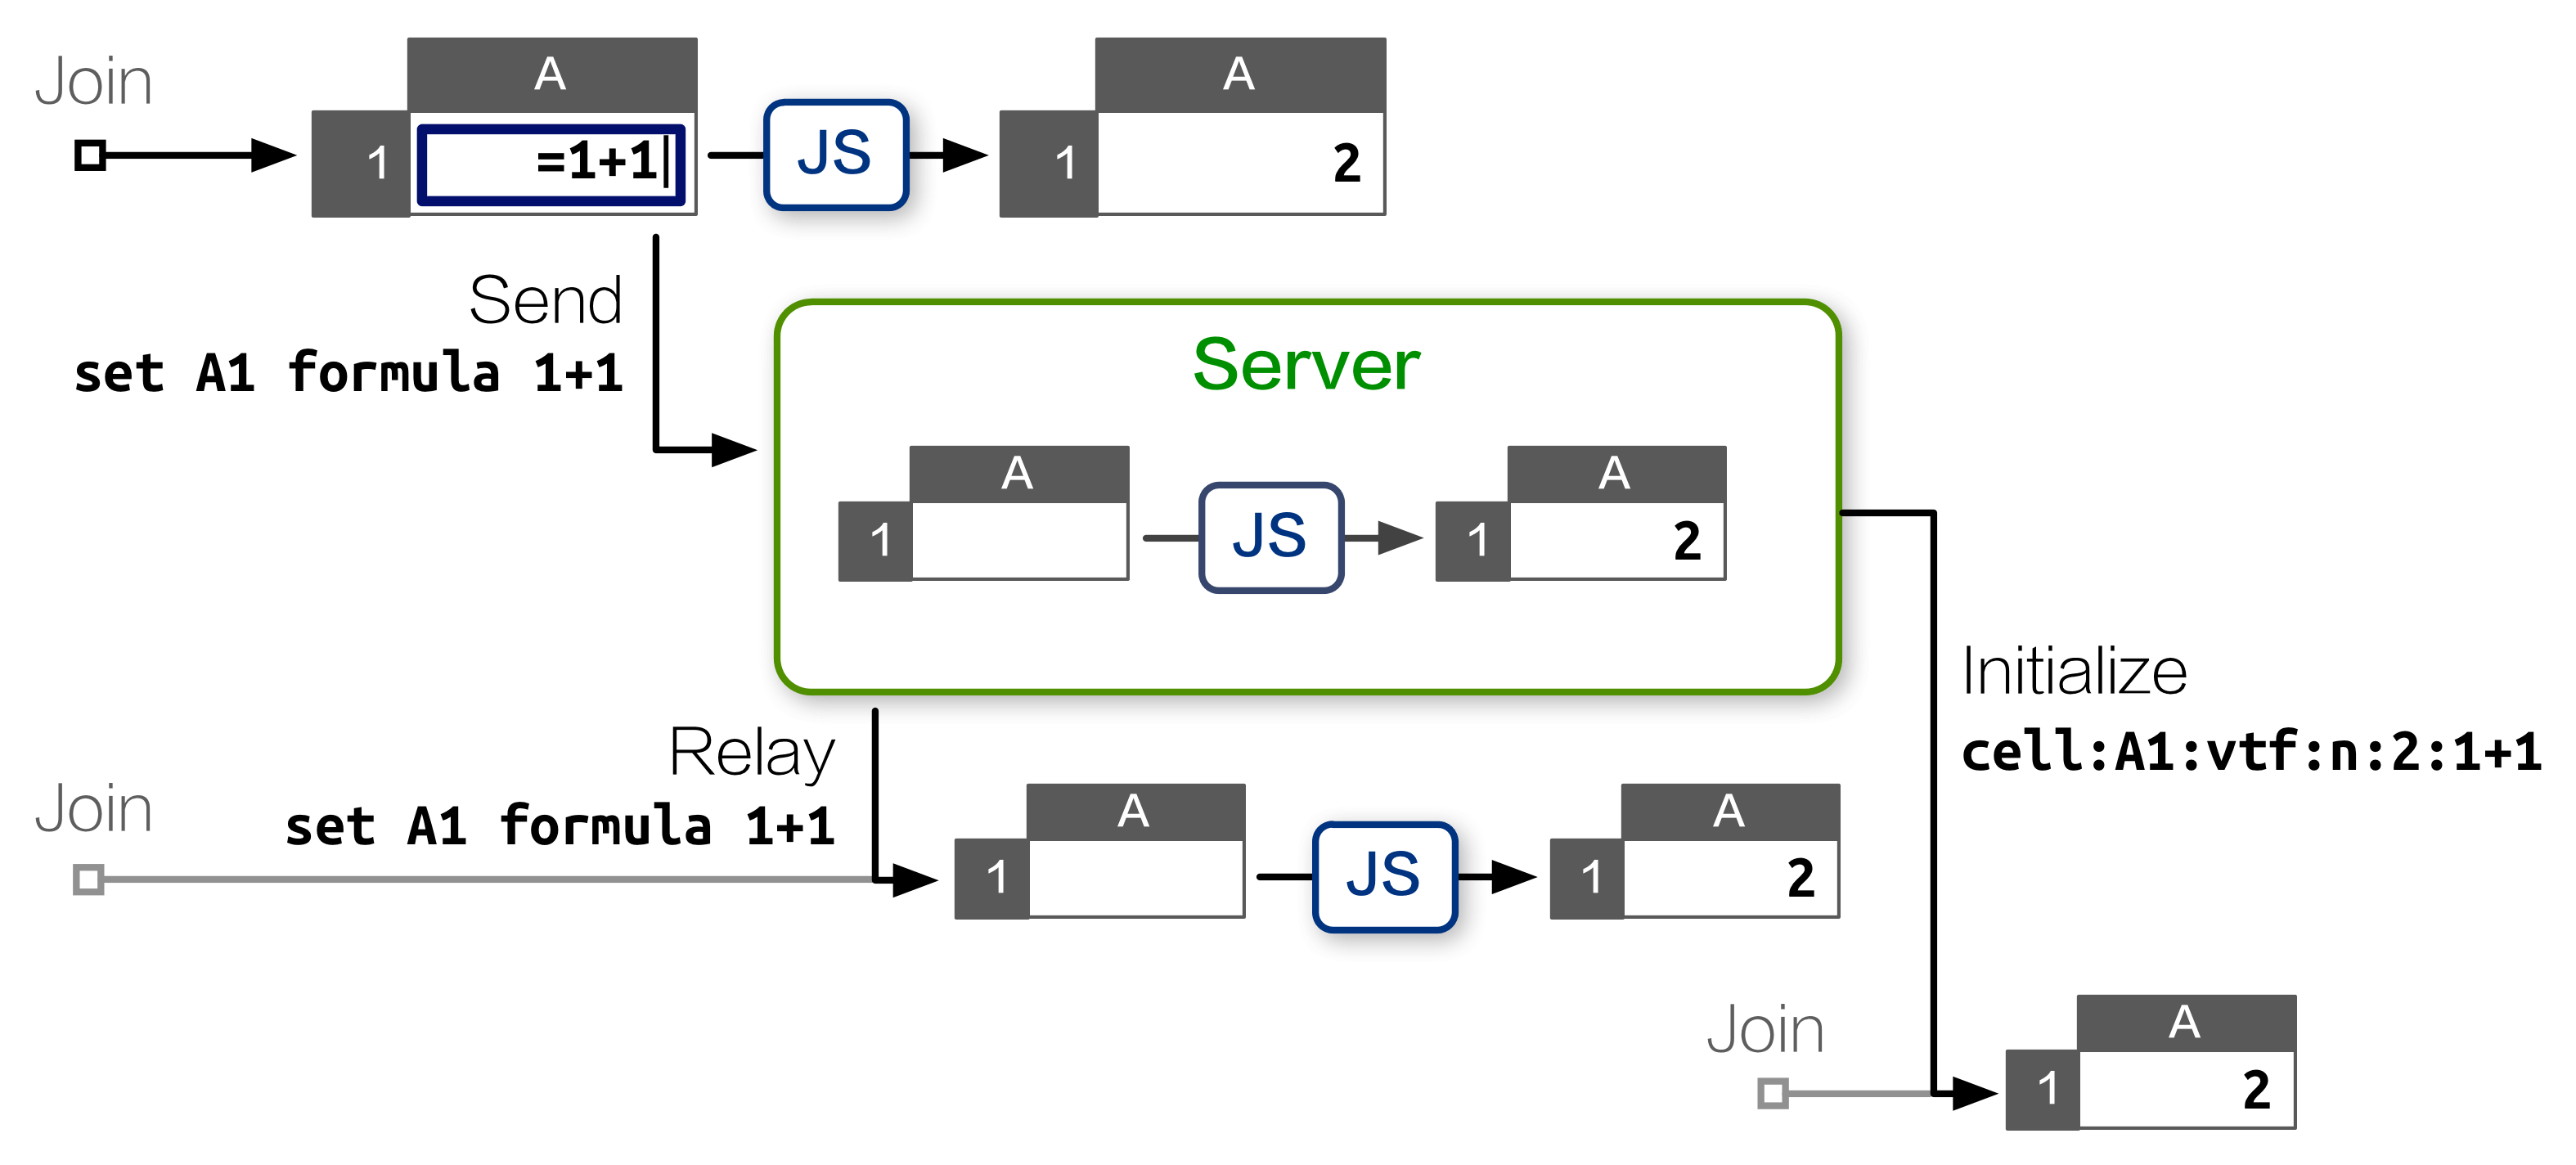
\includegraphics[width=0.6\textwidth]{resources/chapter-2-ethercalc.png}
        \caption{Ilustrasi Cara Kerja Kolaborasi pada EtherCalc}
        \label{IlustrasiEtherCalc}
    \end{figure}

    \subsubsection{Google Sheet}
    Google Sheet merupakan salah satu perangkat lunak pada \textit{office suit} miliki Google. Google Sheet dapat berjalan diatas tiga \textit{platform} yang berbeda yakni: sebagai \textit{web application}, Chrome apps, dan \textit{mobile apps}. Sheet memiliki kemampuan berkolaborasi secara \textit{real-time} dan menyediakan fitur-fitur \textit{spreadsheet} yang ada pada umumnya. Sheet memiliki fitur \textit{revision history} sehingga setiap orang dapat melihat perubahan yang terjadi, \textit{add-ons} yang dapat menambahkan fitur kepada Sheet melalui program yang dibuat oleh komunitas serta fitur \textit{chat} dengan kolaborator. Google Sheet dikembangkan menggunakan bahasa \textit{javascript} yang memberikan kemampuan penyimpanan dan kolaborasi secara \textit{real-time} \parencite{GoogleSheet}.

    \subsubsection{OnlyOffice}
    Merupakan perangkat lunak sebagai \textit{service} yang dikembangkan oleh Ascensio System SIA. OnlyOffice merupakan \textit{office suite} yang berjalan diatas \textit{web application} yang dipadukan dengan sistem \textit{customer relationship management}. OnlyOffice tidak hanya terdiri dari \textit{online office editor} namun juga terdapat fitur managemen dokumen, manajemen proyek, \textit{mail service}, serta manajemen pelanggan seperti kontak, \textit{invoice}, \textit{opportonities}, dan \textit{task}. OnlyOffice ditujukan kepada bisnis yang membutuhkan perangkat lunak yang dapat mengorganisir kebutuhan bisnis didalam satu aplikasi yang saling terintegrasi \parencite{OnlyOffice}. 


\section{Penggunaan \textit{Spreadsheet}}
\textit{Spreadsheet} dapat digunakan untuk melakukan kalkulasi terhadap suatu rumus atau formula yang sulit jika dikalkulasikan dengan cara manual. Selain itu, \textit{spreadsheet} dapat juga digunakan untuk melakukan ramalan terhadap suatu perubahan variabel masukan. Pada perkembangannya, \textit{spreadsheet} memiliki fitur-fitur tambahan seperti visualisasi data dan ekstraksi data penting dari kumpulan data yang ada.

Penelitian tentang penggunaan \textit{spreadsheet} pada bisnis pernah dilakukan sebelumnya pada tahun 2014. Subjek yang diteliti adalah akuntan manajemen \parencite{Bradbard2014}. Pada penelitian tersebut, didapatkan gambaran umum mengenai penggunaan \textit{spreadsheet} secara umum. Menurut hasil penelitian tersebut beberapa fitur yang sering digunakan oleh pengguna \textit{spreadsheet} secara terurut dari yang paling sering digunakan adalah sebagai berikut,

\begin{enumerate}
    \item Menghitung fungsi matematika dasar (tambah, kurang, kali, bagi, dan lainnya)
    \item Mengelola \textit{worksheet} dan \textit{workbook} (menambahkan, menghapus, merubah nama, dan lainnya)
    \item Melakukan perubahan format dasar (menebalkan, memberi garis bawah, format angkat, dan lainnya)
    \item Melakukan pengurutan data, penghitungan subtotal, serta meringkas data
    \item Menggunakan fitur \textit{cell addressing} baik absolut maupun relatif
    \item Penggunaan fungsi kondisi (IF, COUNTIF), fungsi logika (AND, OR), fungsi pencarian (VLOOKUP, HLOOKUP), menautkan \textit{workbook} lain, serta fungsi pembulatan (ROUND, CEILING, FLOOR)
\end{enumerate}

Penggunaan \textit{spreadsheet} sangat bergantung kepada domain bisnis atau organisasi yang menggunakan. Pada bisnis yang berorientasi komersial, \textit{spreadsheet} dapat digunakan sebagai alat bantu perhitungan laba, pengeluaran, investasi, dan pajak. Pada organisasi-organisasi non komersial, \textit{spreadsheet} dapat digunakan sebagai salah satu bentuk basis data yang menangani penyimpanan, pengelolaan, dan pengumpulan data yang mudah dan cepat.

\section{Kesalahan dalam Penggunaan \textit{Spreadsheet}}
\subsection{Kualitas Data}
Kualitas Data (\textit{Data Quality}) adalah tingkat kemampuan data untuk memenuhi kebutuhan penggunaannya (\textit{usage requirement}) sehingga data dapat digunakan dengan baik \parencite{Khatri2010}. Dimensi yang ada pada kualitas data dapat dibagi menjadi:

    \begin{enumerate}
        \item Akurasi, merujuk kepada tingkat kebenaran dari data.
        \item Aktualitas, menunjukan bahwa data yang dicatat merupakan data terbaru.
        \item Kelengkapan, menunjukkan bahwa nilai-nilai yang diperlukan tercatat (tidak hilang).
        \item Kredibilitas, menunjukkan kepercayaan terhadap sumber serta isinya.
    \end{enumerate}

Tingkatan nilai untuk dimensi tersebut dapat berbeda pada setiap kasus yang ada. Contohnya, akurasi 85\% untuk data nama dan alamat dokter merupakan nilai yang cukup baik bagi perusahaan asuransi yang menargetkan doktor sebagai konsumen potensial, namun tidak cukup baik untuk perusahaan obat yang ingin melakukan \textit{recall} terhadap obat yang terdistribusi. Kualitas data yang buruk dapat menyebabkan akibat yang fatal dalam bisnis baik secara operasional maupun strategis. 

\subsection{Tingkat Kesalahan dalam Penggunaan \textit{Spreadsheet}}
Penelitian telah dilakukan oleh Panko \parencite{Panko1998} untuk mengetahui banyaknya kesalahan yang terjadi pada pengembangan \textit{spreadsheet} terutama pada sektor bisnis. Dari penelitian ini, didapatkan bahwa 20\% hingga 40\% \textit{spreadsheet} mengandung kesalahan. Pada kasus tertentu, bahkan ditemukan 90\% \textit{spreadsheet} yang diteliti memiliki kesalahan \parencite{Journal1996}. 

Penelitian yang dilakukan oleh Panko juga menemukan 88\% dari 113 \textit{spreadsheet} yang diaudit melalui 7 lebih studi yang diteliti. Beberapa hasil yang telah di rangkum oleh penelitian tersebut mengunakan \textit{spreadsheet} yang digunakan di dunia nyata dapat dilihat pada Tabel \ref{StudiKesalahan}.
  \begin{longtable}{ | L{3cm} | R{2cm} | R{2cm} | R{2cm} | L{3cm} | }
    \caption{Studi terhadap Kesalahan pada \textit{Spreadsheet}}
    \label{StudiKesalahan}\\ \hline
    \centering\bfseries{Pembuat} & \centering\bfseries{Jumlah yang Diaudit} & \centering\bfseries{Rata-rata Sel} & \centering\bfseries{Persentase Error} & \centering\bfseries{Keterangan Kesalahan} \tabularnewline \hline
    \endfirsthead
    \hline
    \centering\bfseries{Pembuat} & \centering\bfseries{Jumlah yang Diaudit} & \centering\bfseries{Rata-rata Sel} & \centering\bfseries{Persentase Error} & \centering\bfseries{Keterangan Kesalahan} \tabularnewline \hline
    \endhead
    Butler (1992) & 273 & - & 11\% & Kesalahan perhitungan pada pajak\\ \hline
    Dent (1994) & Tidak diketahui & - & 30\% & Menggunakan angka yang ditulis manuals yang mengakibatkan perhitungan berikutnya salah\\ \hline
    Hicks (1995) & 1 & 3856 & 100\% & Kesalahan interpretasi pada data \\ \hline
    Coopers \& Lybrand (1997) & 23 & 150+ & 91\% & Kesalahan perhitungan yang meleset hingga 5\% \\ \hline
    Lukasic (1998) & 2 & 2270 - 7027 & 100\% & Kesalahan akibat melebih-lebihkan perhitungan hingga 16\%\\ \hline
    Clermont, Hanin, \& Mittermeier (2002) & 3 & - & 100\% & Kesalahan akibat perhitungan sel kosong\\ \hline
    Lawrence and Lee (2004) & 30 & 2182 & 100\%  & Kesalahan perhitungan dan formula\\ \hline
    Powell, Lawson, and Baker (2007) & 25 & - & 64\%  & Kesalahan perhitungan dan formula \\ \hline
    Powell, Baker \& Lawson (2007) & 50 & - & 86\%  & Kesalahan perhitungan dan formula \\ \hline
  \end{longtable}
Dari kumpulan data diatas, dapat dilihat bahwa didalam pembentukan \textit{spreadsheet} pada bidang bisnis, tidak mungkin terlepas dari kesalahan. Dengan tingginya tingkat kesalahan ini, bisnis dapat mengalami kerugian secara material maupun moral yang cukup besar \parencite{EUSPRIGHorrorStories}. Hal ini mengindikasikan bahwa tingginya tingkat kesalahan harus dapat diselesaikan agar tidak terjadi kerugian di dalam penggunaan \textit{spreadsheet} terutama dalam bisnis.

\subsection{Tipe Kesalahan dalam Penggunaan \textit{Spreadsheet}}
Tingkat fleksibilitas \textit{spreadsheet} yang tinggi memberikan keleluasaan kepada penggunanya untuk melakukan banyak manipulasi dan pengelolaan data. Tingginya fleksibilitas ini dapat berakibat mudahnya \textit{human error} terjadi pada saat penggunaan \textit{spreadsheet} yang menyebabkan terjadinya kesalahan-kesalahan pada data. Tipe-tipe kesalahan pada \textit{spreadsheet} dapat dibagi menjadi dua jenis tipe kesalahan yakni kesalahan kuantitatif, dan kesalahan kualitatif \parencite{Panko1998}. 

    \subsubsection{Kesalahan Kualitatif}
    Kesalahan kualitatif merupakan kesalahan yang berhubungan dengan kualitas \textit{spreadsheet} tersebut lebih menitikberatkan pada kebiasaan dan prosedur yang salah didalam pembuatan \textit{spreadsheet}. Beberapa kesalahan yang dapat diklasifikasikan sebagai kesalahan kualitatif adalah \parencite{Powell2009}:

    \begin{enumerate}
        \item Melakukan \textit{hard-code} pada suatu angka di dalam formula
        \item Menggunakan formula yang panjang dalam perhitungan
        \item Susunan data yang tidak direncanakan dengan baik
        \item Tidak adanya dokumentasi mengenai \textit{spreadsheet} yang dibuat
    \end{enumerate}

    Kesalahan ini tidak langsung mengakibatkan nilai hasil keluaran yang salah namun menurunkan kualitas dari \textit{spreadsheet} tersebut \parencite{Rajalingham2001}. Selain itu, kesalahan kualitatif dapat menyebabkan kesalahan kuantitatif terutama pada saat penggunaan fungsi analisis \textit{what-if} pada \textit{spreadsheet} \parencite{Panko1998}.

    \subsubsection{Kesalahan Kuantitatif}
    Kesalahan ini mengakibatkan \textit{spreadsheet} mengeluarkan hasil dan nilai yang salah didalam operasi perhitungannya. Kesalahan kuantitatif dapat dibagi menjadi tiga tipe kesalahan yakni \parencite{Panko1998}:

    \begin{enumerate}
        \item Kesalahan mekanikal (\textit{mechanical error}) yang biasanya terjadi akibat kesalahan pengetikan angka atau rujukan sel yang salah pada suatu formula
        \item Kesalahan logika (\textit{logical error}) yang terjadi pada pembuatan formula yang salah atau penggunaan fungsi yang tidak tepat
        \item Kesalahan akibat kelalaian pada interpretasi situasi atau spesifikasi yang diberikan sehingga \textit{spreadsheet} yang dihasilkan tidak sesuai dengan domain permasalahan yang ada atau \textit{ommision error} \parencite{Powell2009}
    \end{enumerate}

\subsection{Penanganan Kesalahan pada \textit{Spreadsheet}}
Berdasarkan penelitian yang dilakukan oleh Panko \parencite{Panko1998}, dijabarkan beberapa metode untuk menangani dan mengurangi kesalahan yang sering terjadi. Beberapa metode yang dapat digunakan yakni:

    \begin{enumerate}
        \item Membangun \textit{preliminary design} sebelum pembuatan \textit{spreadsheet} agar terdapat perencanaan yang baik di dalam pembangunan data di dalam \textit{spreadsheet}
        \item Melakukan proteksi terhadap sel yang tidak boleh diubah.
        \item Melakukan pengecekan terhadap semua rumus dan formula yang dimasukan bahkan hingga rumus yang cukup sederhana dengan cara melakukan pengecekan manual.
        \item Membuat dokumentasi untuk \textit{spreadsheet} yang dibuat.
        \item Tidak menekan pembuat \textit{spreadsheet} terhadap kesalahan yang dibuat dengan memberikan hukuman. Kesalahan yang terjadi pada \textit{spreadsheet} umumnya masih berada pada batas normal \textit{human error} sehingga memberikan hukuman akan membuat rasa takut dalam melaporkan kesalahan.
        \item Melakukan inspeksi terhadap formula, rumus, dan kode yang dibuat baik oleh individual maupun secara berkelompok.
    \end{enumerate}

\section{Data pada \textit{Spreadsheet}}

\subsection{Tipe Struktur Data pada \textit{Spreadsheet}}
Pada penelitian yang dilakukan oleh Chen dan Cafarella, \textit{spreadsheet} dapat dibagi menjadi 2 jenis yakni; \textit{data frame} dan \textit{non-data frame}. \textit{Data frame} merupakan tipe \textit{spreadsheet} yang terdiri dari 2 komponen utama: area nilai dan area atribut atau metadata (biasanya berada di atas dan atau di kiri area nilai). \textit{Non-data frame} adalah tipe \textit{spreadsheet} selain tipe \textit{data frame} yang telah didefinisikan sebelumnya. Tipe \textit{non-data frame} dapat dibagi menjadi beberapa jenis yakni:

    \begin{enumerate}
        \item Relasi merupakan tipe \textit{spreadsheet} yang dapat langsung diubah ke model relasional.
        \item Formulir merupakan \textit{spreadsheet} yang tidak ditujukan sebagai penyimpanan dan didesain untuk diisi oleh manusia.
        \item Diagram yang digunakan sebagai visualisasi data, biasanya berisi banyak data tanpa skema informasi yang detil.
        \item Daftar atau \textit{List} merupakan catatan sejumlah nama atau hal (tentang kata-kata, nama orang, barang, dan sebagainya) yang disusun berderet dari atas ke bawah \parencite{pusat1991kamus}.
        \item Jadwal merupakan \textit{spreadsheet} digunakan sebagai pembuatan dan pengelolaan jadwal.
        \item Silabus merupakan kerangka unsur kursus pendidikan, disajikan dalam aturan yang logis, atau dalam tingkat kesulitan yang makin meningkat \parencite{pusat1991kamus}.
        \item \textit{Scorecard} yakni suatu alat manajemen yang biasanya berguna untuk membantu manajer melacak aktivitas yang dilakukan oleh stafnya.
    \end{enumerate}

Penelitian ini menggunakan sampel 200 \textit{spreadsheet} yang dilabeli oleh ahli dan didapatkan bahwa 50.5\% \textit{spreadsheet} merupakan tipe \textit{data frame}, dimana 32.5\% memiliki label atribut dibagian atas atau bawah. Sedangkan 49.5\% \textit{spreadsheet} bertipe \textit{non-data frame} terdiri dari 22.0\% relasi, 10.5\% formulir, 3.5\% diagram, 3\% berupa \textit{list}, dan 10.5\% lainnya \parencite{Chen2013}.

\subsection{Pengolahan Data pada \textit{Spreadsheet}}
    \subsubsection{\textit{Extract-Transform-Load} (ETL)}
    \textit{Extract-Transform-Load} (ETL) adalah proses yang digunakan sebagai metode integrasi data dari beberapa sumber dan aplikasi. ETL biasanya digunakan pada saat melakukan proses \textit{data warehouse} dimana data dari sumber eksternal diambil, lalu ditransformasikan ke bentuk yang sesuai dengan kebutuhan (didalam prosesnya bisa terkadung pengecekan kualitas), dan memasukannya ke dalam basisdata yang telah ditentukan \parencite{Bansal2014}. Terdapat tiga fase pada proses ETL yakni:

    \begin{enumerate}
        \item \textit{Extract}, fase pertama ini adalah proses yang melakukan ekstraksi data dari sumber yang dipilih. Data biasanya tersedia didalam format \textit{flat file} seperti csv, xls, dan txt atau melalui klien RESTful.
        \item \textit{Transform}, pada fase ini data dibersihkan agar sesuai dengan skema tujuan. Beberapa cara untuk mentransformasikan data adalah dengan menormalisasi data, menghapus duplikasi, melakukan pengecekan terhadap batasan-batasan, melakukan \textit{filtering}, melakukan pengurutan dan pengelompokan, atau fungsi-fungsi lain yang didefinisikan.
        \item \textit{Load}, pada fase ini data yang telah ditransformasikan dimasukan ke dalam \textit{data mart} atau \textit{data warehouse} yang ditentukan.
    \end{enumerate}

    \subsubsection{Metode ETL pada \textit{Spreadsheet}}
    Pada penelitian yang dilakukan oleh Chen, pengolahan data pada sebuah \textit{spreadsheet} bertipe \textit{data frame} dapat dibagi menjadi tiga proses yakni: \textit{frame finder}, \textit{hierarchy extractor}, dan \textit{tuple builder}. Proses \textit{frame finder} dilakukan dengan cara mengidentifikasi \textit{data frame} serta mencari lokasi dari atribut dan nilai. Pada proses \textit{hierarchy extractor}, atribut yang ada pada \textit{data frame} yang ditemukan dicari hirarkinya setelah itu proses \textit{tuple builder} membentuk \textit{tuple} relasional untuk setiap nilai yang ada. Proses ini tidak membedakan \textit{spreadsheet} tipe \textit{data frame} atau bukan, sehingga diasumsikan jika \textit{tuple} yang dihasilkan memiliki kualitas yang baik, dapat dikatakan bahwa \textit{spreadsheet} masukan bertipe \textit{data frame} dan sebaliknya. \parencite{Chen2013}

        \paragraph{\textit{Frame Finder}}
        Tujuan dari proses \textit{frame finder} adalah mengidentifikasi wilayah nilai dan wilayah atribut yang dapat berupa \textit{left attribute} maupun \textit{top attribute}. Untuk mensimplifikasi permasalahan, Chen menganggap bahwa \textit{data frame} tidak akan berada sejajar secara horisontal, namun hanya secara vertikal. Sehingga proses ini dapat disimplifikasi menjadi labeling terhadap baris per baris. Label yang akan diberikan adalah \textit{title}, \textit{header}, \textit{data}, dan \textit{footnote}.

        Pelabelan dapat dilakukan dengan algoritma \textit{conditional random field} (CRF) karena terdapat keterkaitan antara satu baris terhadap baris yang lain didalam penggunaan baris. Contohnya, jika baris telah teridentifikasi sebagai \textit{header}, maka besar kemungkinan bahwa baris selanjutnya adalah \textit{data} atau \textit{header}. CRF memiliki kemampuan untuk melakukan \textit{machine learning} yang memperhitungkan label pada elemen sebelumnya.

        \paragraph{\textit{Hierarcy Extractor}}
        Proses ini bertujuan untuk mendapatkan hirarki dari atribut-atribut yang ada. Masukan dari proses ini adalah \textit{data frame} dengan \textit{top attribute} dan \textit{left attribute} dan keluarannya berupa hirarki untuk masing-masing atribut atas dan kiri tersebut. Proses ini dapat dilakukan melalui dua algoritma: \textit{classification} dan \textit{enforced-tree classification}.

        \textit{Classification} dilakukan dengan cara berbeda untuk \textit{left attribute} dan \textit{top attribute}. Pada \textit{left attribute}, klasifikasi dapat dilakukan dengan dua cara: pengecekan terhadap \textit{formatting} pada sebuah sel dan kedekatan sel secara geometris. Semakin mirip \textit{formatting} sebuah sel, maka semakin mungkin bahwa kedua sel bukan merupakan pasangan \textit{parent} dan \textit{child} dan semakin dekat sel secara geometris, kemungkinan kedua sel meruapakan  pasangan \textit{parent} dan \textit{child} semakin besar. Sedangkan pada \textit{top attribute} dapat dilakukan pengecekan posisi antar baris atribut bagian atas.

        Kelemahan pada metode klasifikasi sebelumnya adalah terdapat kemungkinan tidak dapat dibentuk pohon dari hasil klasifikasi. \textit{Enforced-tree classification} mencoba untuk menyelesaikan permasalahan ini dengan dua langkah tambahan yakni: memastikan bahwa suatu atribut hanya dapat memiliki satu \textit{parent} dimana yang terpilih menjadi \textit{parent} adalah atribut dengan probabilitas tertinggi, dan memastikan bahwa tidak ada \textit{cycle} yang terbentuk dengan cara menghapus keterhubungan dengan nilai probabilitas terkecil. Klasifikasi ini tetap menggunakan metode klasifikasi fitur yang dilakukan pada algoritma \textit{classification}.

        \paragraph{\textit{Tuple Builder}}
        Proses ini dilakukan dengan cara mengiterasi setiap \textit{value (v)} dan mencari atribut akar pada atribut bagian kiri dan atas dari \textit{v}. Setelah dibentuk \textit{relational tuple} untuk nilai \textit{v} dengan atribut bagian kiri dan atas tersebut. Tingkat akurasi dari proses ini sangat bergantung dari dua proses sebelumnya.

% \section{\textit{Data Governance}}
% Penggunaan \textit{spreadsheet} pada bisnis tidak terlepas dari adanya penyimpanan dan pengelolaan informasi. 

\section{Studi dan Penelitian Terkait}
    \subsection{\textit{Senbazuru: A Prototype Spreadsheet Database Management System}}
    Senbazuru \parencite{Chen2013-2} merupakan prototipe yang dikembangkan dengan tujuan untuk mempermudah pencarian, pengaksesan, pengubahan, dan melakukan \textit{query} terhadap \textit{spreadsheet}. Pengembangan ini ingin menyelesaikan permasalahan dimana data \textit{spreadsheet} sangat tersebar diberbagai tempat sehingga untuk mendapatkan informasi yang diinginkan atau membandingkan antar informasi di dalam beberapa \textit{spreadsheet} sangatlah sulit. 

    Didalam pengembangan prototipe ini, kesulitan teknikal yang harus dihadapi adalah proses ekstraksi dan perbaikan data. Didalam melakukan ekstraksi data, harus dilakukan beberapa proses berikut: mendeteksi mana atribut dan nilai, mengidentifikasi hirarki atribut, membentuk \textit{relational tuple}, dan membentuk \textit{tuple} tersebut menjadi tabel relasional. Dari hasil dari ekstrasi ini, masih sangat mungkin memiliki kesalahan sehingga proses perbaikan diperlukan didalam pembentukan tabel relasional ini. Proses perbaikan pada protitipe ini dilakukan manual dengan bantuan pengguna.

    \subsubsection{Arsitektur Sistem}

    \textit{Spreadsheet Database Maanagement System} (SSDBMS) yang dikembangkan pada prototipe ini memiliki tiga proses utama yakni: \textit{search}, \textit{extract}, dan \textit{query}. Proses pencarian dilakukan terhadap repositori \textit{spreadsheet} yang ada di internet, lalu data \textit{spreadsheet} tersebut diekstraksi dan dijadikan tabel relasional, dan setelah itu pengguna dapat melakukan \textit{query} terhadap tabel yang telah dibentuk.

        \paragraph{\textit{Search}}
        Komponen pencarian ini memudahkan pengguna untuk menemukan dataset yang tepat menggunakan bantuan internet. Saat prototipe ini dikembangkan, Senbazuru telah mengindeks 1800 \textit{spreadsheet} yang didapatkan dari U.S. Census Bureau. Pengindeksan menggunakan bantuan \textit{library} Python yakni xlrd untuk mengekstraksi teks dari sel lalu menggunakan Apache Lucene untuk melakukan indeks pada teks. Pencarian menggunakan metode \textit{term frequency–inverse document frequency} (TF-IDF) untuk mendapatkan relevansi dokumen.
        
        \paragraph{\textit{Extract}}
        Proses ekstraksi data pada \textit{spreadsheet} dilakukan melalui empat tahapan yakni:

        \begin{enumerate}
            \item \textit{Frame Finder}

            Tahap ini dilakukan untuk mencari \textit{frame} pada \textit{spreadsheet} bertipe \textit{data frame}. Dengan menggunakan algoritma \textit{conditional random field} (CRF) untuk memberikan label pada setiap baris yang tidak kosong pada \textit{spreadsheet}. Tahap ini akan menghasilkan \textit{data frame} yang selanjutnya akan digunakan pada tahap selanjutnya, baris lain yang dianggap bukan \textit{data frame} akan diabaikan.

            \item \textit{Hierarchy Extractor}
            
            Tahap selanjutnya adalah ekstraksi hirarki pada wilayah atribut dari \textit{data frame} yang ditemukan. Pada setiap atribut, akan dicari atribut mana yang dideskripsikan oleh atribut lainnya dan seterusnya hingga terbentuk hirarki dari atribut-atribut yang ada. Kesalahan pada pembentukan hirarki sangat mungkin terjadi sehingga pengguna akan diberikan kemampuan untuk memperbaiki hirarki yang salah pada bagian \textit{repair interface}. Setelah perbaikan dilakukan oleh pengguna, Senbazuru akan menjalankan kembali CRF untuk melakukan pembelajaran terhadap label baru yang diberikan.

            \item \textit{Tuple Builder}
            
            Bagian ini melakukan pembentukan \textit{tuple} antara wilayah nilai dan wilayah atribut yang sesuai.

            \item \textit{Relation Constructor}

            Tahap ini melakukan transalasi dari \textit{tuple} yang terbentuk menjadi tabel relasional dengan cara membentuk kluster terhadap atribut yang satu jenis. Contohnya, terdapat atribut \textit{Male}, \textit{total}, dan \textit{Female}, ketiga atribut tersebut memiliki jenis yang sama sehingga harus digabungkan menjadi satu kolom yakni \textit{gender}. Pada Senbazuru, teknik pengklusteran ini menggunakan bantuan koleksi skema dari Freebase dan YAGO.
        \end{enumerate}

        \paragraph{\textit{Query}}
        Setelah proses sebelumnya selesai, maka pengguna dapat memasukan perintah relasional terhadap data \textit{spreadsheet} yang telah diubah menjadi tabel relasional. Pada prototipe yang dikembangkan, perintah yang diimplementasikan adalah \textit{join} dan \textit{select}.

    \subsubsection{Kesimpulan Penelitian}
    Senbazuru merupakan prototipe untuk manajemen basis data berbasis \textit{spreadsheet} yang dapat melakukan pencarian data pada internet melalui kata kunci yang diberikan. Prototipe ini berhasil melakukan ekstraksi data secara otomatis walaupun tidak terlepas dari kesalahan. Kesalahan yang terjadi masih harus seringkali dilakukan perbaikan secara manual. Namun dengan penggunaan algoritma CRF, protitipe dapat mengurangi kesalahan yang terjadi. Prototipe ini juga ditujukan sebagai demo kepada peserta konferensi VLDB dan diharapkan dapat menarik perhatian komunitas basis data.

\subsection{\textit{Spreadsheet As a Relational Database Engine}}
Penelitian \parencite{Tyszkiewicz2010} pernah dilakukan terhadap pembuatan \textit{spreadsheet} menjadi mesin basis data relasional. Penelitian ini dilatarbelakangi dengan tingginya penggunaan \textit{spreadsheet} pada banyak bidang dan kurangnya kualitas data yang ada didalamnya yang dapat menyebabkan kesalahan-kesalahan terjadi pada perhitungan dan prediksi. Solusi yang dipaparkan pada penelitian ini adalah dengan menggabungkan \textit{spreadsheet} dan \textit{database engine} dengan menggunakan formula sebagai ganti dari \textit{SQL query}.

    \subsubsection{Arsitektur Sistem}

    Pada implementasinya, sebuah \textit{workbook} akan memiliki satu \textit{worksheet} untuk setiap tabel data dan satu \textit{worksheet} untuk setiap \textit{view} pada basis data. Dengan menggunakan \textit{external compiler} yang menerima masukan berupa SQL yang akan mengubahnya kedalam bentuk \textit{spreadsheet}. Program tersebut akan mengubah SQL menjadi beberapa formula yang diterima oleh \textit{spreadsheet} tersebut.

    Terdapat dua bagian utama pada \textit{spreadsheet} hasil implementasi yakni: tabel data dan bagian \textit{view}. Bagian tabel data adalah tempat pengguna untuk memasukkan, mengubah, serta menghapus data. Secara teori, bagian tabel data tidak memiliki formula, namun didalam implementasinya mengikuti implementasi SQL dimana perlu dilakukan validasi data dan verifikasi terhadap \textit{primary key}, \textit{foreign key}, dan batasan lain yang ada diperintah \textit{create table}. 

    Bagian \textit{view worksheet} tidak dapat diubah oleh pengguna dan berisikan formula-formula yang independen terhadap data yang dimasukkan oleh pengguna. Selain itu, bagian \textit{view} berisikan kolom-kolom yang berguna sebagai \textit{intermediate result} yang selanjutnya akan digunakan oleh formula lain. Pada awalnya sel-sel akan berisikan "" yang merepresentasikan sel yang belum digunakan.

    \subsubsection{Kesimpulan Penelitian}

    Excel dan \textit{spreadsheet} lain tidak didesain untuk menjadi \textit{database engine} sehingga kebanyakan formula akan dilakukan menggunakan \textit{linear scan} dan hal ini dapat mengurangi performansi. Beberapa cara untuk meningkatkan performansi adalah mengeksploitasi \textit{lazy evaluation} dari \textit{if statement}, mengkomputasi hanya beberapa sel tetangga yang berkaitan, serta menggunakan file atau \textit{workbook} lain untuk membagi \textit{query} dan membangkitkannya ketika dibutuhkan.

    Pada tes perfomansi yang dilakukan pada penelitian ini dapat disimpulkan bahwa untuk operasi dasar dan \textit{query} sederhana penggunaan \textit{spreadsheet} dapat digunakan dengan baik dengan waktu yang cukup cepat. Tingkat efektifitas penggunaan pada arsitektur ini cukup rendah, namun hasil tes tersebut menunjukan bahwa arsitektur ini memiliki potensial yang dapat dikembangkan.
    \chapter{Analisis Masalah Penangganan Kesalahan Pada \textit{Spreadsheet}}
Pada bab ini akan diuraikan analisis persoalan penangganan kesalahan pada \textit{spreadsheet} yang telah diuraikan pada Bab I. Hasil dari bab ini digunakan untuk merancang aplikasi yang akan diimplementasikan seperti yang dijelaskan pada Bab IV.

\section{Model Interaksi Pengguna}
Di dalam pembangunan perangkat lunak \textit{spreadsheet} untuk mengurangi kesalahan, dapat diidentifikasikan dua model interaksi yang dapat diimplementasi. Model interaksi yang pertama adalah menggunakan formulir sebagai basis masukan data dan model yang kedua adalah menggunakan aplikasi \textit{spreadsheet} secara langsung sebagai media input data.

\subsection{Berbasis Formulir}


\subsection{Berbasis \textit{Spreadsheet}}

\section{}

\section{Penentuan Bagian Data dan Label}
\subsection{Manual oleh Pengguna}

\subsection{Secara Otomatis}
Pada penggunaan \textit{spreadsheet}, terutama pada tipe \textit{data frame}, terdapat dua jenis bagian inti yang selalu ada pada \textit{spreadsheet} yakni bagian label dan data. Label merupakan penjelasan dari suatu data. Seperti yang telah dijelaskan pada Subbab \ref{Metode Pencarian}, mekanisme untuk mengidentifikasi label dan data dapat dilakukan melalui 3 tahapan yakni, \textit{frame finder}, \texit{hierarchy extractor}, dan \textit{tuple builder}.

\section{Identifikasi Domain Data Masukan Pengguna}
\subsection{Ditentukan oleh Sistem}

\subsection{Ditentukan oleh Pengguna}


\section{Auto-commit atau Commit-push type?}

\section{Pengecekan Integrasi dan Kesesuaian Data}



\section{Penyimpanan dan Pemulihan Data}



====




\section{Analisis Permasalahan Pada \textit{Spreadsheet}}
\blindtext
Masukin yang versioning, data validatoin (type validation: int, string, date dll), database alternative, make use of DB ACID
http://www.mrc-productivity.com/blog/2012/11/spreadsheet-misuse-why-it-happens-and-how-to-stop-it/
http://www.burns-stat.com/documents/tutorials/spreadsheet-addiction/
Lebih cocok menangani permasalahan misuse spreadsheet sebagai basis data


\section{ Umum}
\blindtext

\section{Rancangan Solusi}
\blindtext
    \chapter{Rancangan, Implementasi, dan Pengujian}

\section{Perancangan Perangkat Lunak} \label{PerancanganPL}
Subbab perancangan perangkat lunak menjelaskan deskripsi aplikasi, analisis kebutuhan fungsional dan non-fungsional, desain perangkat lunak, serta interaksinya.

	\subsection{Deskripsi Umum Aplikasi}
	Aplikasi pengumpulan data yang dibuat merupakan pengembangan terhadap aplikasi \textit{spreadsheet} kolaboratif yang sudah ada sebelumnya yakni EtherCalc. Aplikasi yang ditambahkan ini yang akan melakukan pengaturan koneksi ke basis data. Saat pengguna menginginkan penyimpanan data ke dalam basis data yang dituju, aplikasi ini akan melakukan pencarian bagian label dan data dan melakukan validasi masukan sebelum memasukkan data ke dalam basis data. 

	\subsection{Spesifikasi Kebutuhan}
	Pada subbab ini akan dipaparkan \textit{use case} aplikasi yang akan dibuat serta kebutuhan fungsional dan non-fungsional dari aplikasi. Kasus penggunaan oleh pengguna diberi ID dengan format UC-XX dengan UC menyatakan \textit{use case} dan XX menyatakan nomor. Pengguna adalah pihak yang menggunakan aplikasi \textit{spreadsheet} yang sudah ditambahkan fitur pengumpulan data. Kasus penggunaan oleh pengguna dijelaskan pada Tabel \ref{KebutuhanPengguna}.

	\begin{small}
	\begin{longtable}{ | p{2cm} | p{10cm} | }
	    \caption{Kasus Penggunaan oleh Pengguna}
	    \label{KebutuhanPengguna}\\ \hline
	    \centering\bfseries{ID} & \centering\bfseries{Keterangan} \tabularnewline \hline
	    \endfirsthead
	    \hline
	    \centering\bfseries{ID} & \centering\bfseries{Keterangan} \tabularnewline \hline
	    \endhead
	    UC-01 & Pengguna dapat menentukan basis data tujuan dengan konfigurasi basis data yang diinginkan. \\ \hline
	    UC-02 & Pengguna dapat menyimpan data yang dikumpulkan ke dalam basis data pada saat dibutuhkan. \\ \hline
	    UC-03 & Pengguna dapat menambah dan mengurangi tabel yang ingin disimpan secara manual maupun otomatis. \\ \hline
	    UC-04 & Pengguna dapat memperbaiki atribut tabel yang ingin disimpan. \\ \hline
	    UC-05 & Pengguna dapat memberikan batasan dan validasi pada suatu domain data. \\ \hline
	\end{longtable}
	\end{small}

	Berdasarkan kasus penggunaan di atas, dirancang kebutuhan fungsional perangkat lunak yang diberi ID dengan format FR-XX dengan FR merupakan singkatan dari \textit{functional requirement} dan XX menyatakan nomor kebutuhan. Kebutuhan fungsional dijelaskan pada Tabel \ref{KebutuhanFungsional}.

	\begin{small}
	\begin{longtable}{ | p{2cm} | p{6cm} | p{4cm} | }
	    \caption{Kebutuhan Fungsional Aplikasi}
	    \label{KebutuhanFungsional}\\ \hline
	    \centering\bfseries{ID} & \centering\bfseries{Keterangan} & \centering\bfseries{ID Use Case Terkait} \tabularnewline \hline
	    \endfirsthead
	    \hline
	    \centering\bfseries{ID} & \centering\bfseries{Keterangan} & \centering\bfseries{ID Use Case Terkait} \tabularnewline \hline
	    \endhead
	    FR-01 & Aplikasi dapat melakukan koneksi kepada basis data yang ditentukan oleh pengguna melalui data masukan berupa \textit{host}, \textit{port}, \textit{username}, \textit{password}, dan \textit{database} dari basis data yang dituju. & UC-01 \\ \hline
	    FR-02 & Aplikasi dapat melakukan perintah basis data kepada basis data yang dituju. & UC-01, UC-02 \\ \hline
	    FR-03 & Aplikasi menyediakan tombol untuk melakukan \textit{commit} terhadap data yang akan disimpan. & UC-02 \\ \hline
	    FR-04 & Aplikasi menyediakan fitur menambah dan mengurangi tabel baik secara pendeteksian otomatis maupun manual. & UC-03 \\ \hline
	    FR-05 & Aplikasi dapat menampilkan hasil identifikasi label dan data dalam bentuk tabel. & UC-03, UC-04 \\ \hline
	    FR-06 & Aplikasi menyediakan fitur bagi pengguna agar dapat mengubah hasil identifikasi label dan data. & UC-04 \\ \hline
	    FR-07 & Aplikasi menyediakan fitur bagi pengguna agar dapat menambahkan batasan masukan pada suatu data. & UC-05 \\ \hline
	    FR-08 & Aplikasi dapat melakukan validasi data masukan sesuai dengan batasan yang diberikan oleh pengguna. & UC-05 \\ \hline
	    FR-09 & Aplikasi dapat memberitahukan kesalahan validasi yang terjadi. & UC-05 \\ \hline
	\end{longtable}
	\end{small}

	Selain kebutuhan fungsional, dijabarkan juga kebutuhan non-fungsional yang memiliki ID dengan format NF-XX dengan NF merupakan singkatan dari \textit{non-functional requrirement} dan XX menyatakan nomor. Kebutuhan non-fungsional disajikan pada Tabel \ref{KebutuhanNonfungsional}.

	\begin{small}
	\begin{longtable}{ | p{2cm} | p{6cm} | p{4cm} | }
	    \caption{Kebutuhan Non-fungsional Aplikasi}
	    \label{KebutuhanNonfungsional}\\ \hline
	    \centering\bfseries{ID} & \centering\bfseries{Keterangan} & \centering\bfseries{ID Use Case Terkait} \tabularnewline \hline
	    \endfirsthead
	    \hline
	    \centering\bfseries{ID} & \centering\bfseries{Keterangan} & \centering\bfseries{ID Use Case Terkait} \tabularnewline \hline
	    \endhead
	    NF-01 & Data masukan pengguna disimpan secara persisten. & UC-01, UC-02 \\ \hline
	    NF-02 & Aplikasi dapat berjalan diatas aplikasi \textit{spreadsheet} EtherCalc. & - \\ \hline
	    NF-03 & Laporan hasil pencatatan \textit{response time} fitur yang ditambahkan. & - \\ \hline
	\end{longtable}
	\end{small}

	\subsection{Kebutuhan Modul} \label{KebutuhanModul}
	Pembangunan fitur ini diatas aplikasi EtherCalc terdiri dari lima buah modul, yaitu:
	\begin{enumerate}
		\item Modul \texttt{player}, bertugas sebagai jembatan antara \textit{front-end} dan \textit{back-end} dari fitur.
		\item Modul \texttt{mysql}, bertugas untuk antarmuka baca tulis basis data.
		\item Modul \texttt{framefinder}, bertugas untuk mendeteksi secara otomatis bagian label dan data pada tabel.
		\item Modul \texttt{hierarchyfinder}, bertugas untuk mendeteksi secara otomatis tabel-tabel yang ada dalam suatu \textit{sheet}.
		\item Modul \texttt{table}, bertugas untuk mengelola tabel konfigurasi, melakukan validasi data, dan membuat representasi relasional.
	\end{enumerate}

	Ketergantungan antar modul dapat dilihat pada Gambar \ref{ModuleDependency}

	\begin{figure}[htb]
	    \centering
	    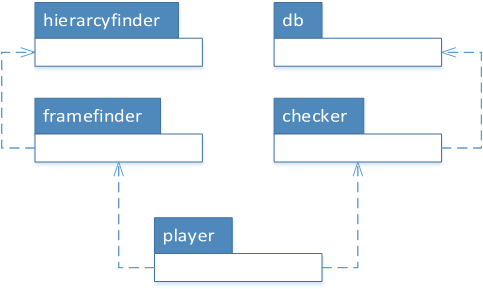
\includegraphics[width=0.4\textwidth]{resources/chapter-4-module-dependecy.png}
	    \caption{Ketergantungan Antar Modul}
		\label{ModuleDependency}
	\end{figure}

	\subsection{Kolaborasi Antar Modul}
	Proses fitur ini akan dilakukan melalui modul \texttt{player} yang dapat menerima perintah pengguna melalui \textit{front-end}. Selanjutnya modul \texttt{framefinder} akan melakukan pendeteksian label dan data secara otomatis pada masing-masing tabel yang terdapat pada \textit{sheet}. Tabel-tabel tersebut didapatkan melalui modul \texttt{hierarchyfinder}. Selanjutnya, pada saat menerima perintah penyimpanan, modul \texttt{table} akan dipanggil oleh \texttt{player}. Jika data masukan sudah benar, maka modul \texttt{mysql} akan melakukan pennyimpanan ke dalam basis data. Kolaborasi antar modul disajikan pada Gambar \ref{ModuleFlow}.

	\begin{figure}[htb]
	    \centering
	    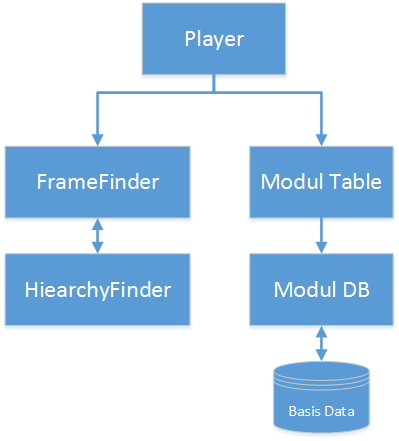
\includegraphics[width=0.5\textwidth]{resources/chapter-4-module-flow.png}
	    \caption{Kolaborasi Antar Modul}
		\label{ModuleFlow}
	\end{figure}

	Pada aplikasi Ethercalc, modul yang ditambahkan akan berada di bawah modul \texttt{player} yang sudah ada. Ilustrasi penempatan modul yang dibuat pada aplikasi EtherCalc yang sudah ada dapat dilihat pada Gambar \ref{ModulePlacing}.

	\begin{figure}[htb]
	    \centering
	    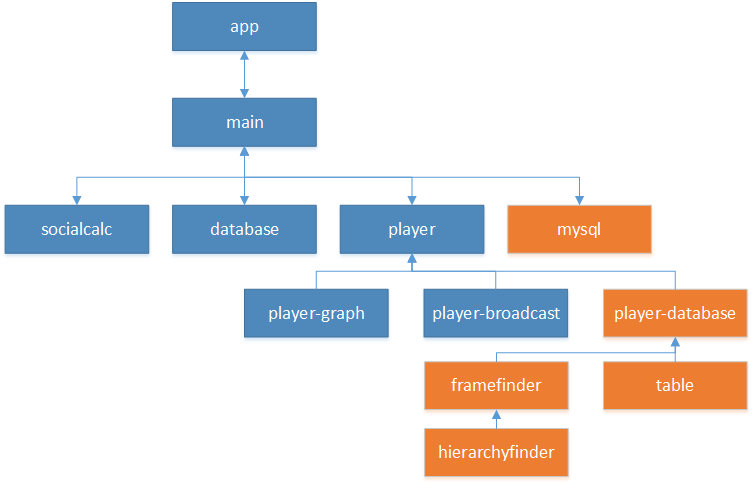
\includegraphics[width=0.6\textwidth]{resources/chapter-4-module-placing.png}
	    \caption{Interaksi dengan Modul yang Sudah Ada}
		\label{ModulePlacing}
	\end{figure}

	\subsection{Arsitektur}
	Aplikasi dibuat dengan menggunakan bantuan Docker sehingga diharapkan dapat dengan mudah dipasang pada berbagai \textit{platform}. Aplikasi terdiri dari tiga \textit{docker container} yakni untuk aplikasi utama, basis data redis, dan basis data MySQL. \textit{File} \texttt{docker-compose.yml} yang dibuat untuk mendefinisikan \textit{docker container} yang digunakan dapat dilihat pada Kode \ref{KodeCompose}

	\begin{lstlisting}[frame=single, basicstyle=\linespread{1}\scriptsize\listingsfont, captionpos=b, caption={Kode pada docker-compose.yml}, label=KodeCompose]
	ethercalc:
	  build: .
	  ports:
	    - "80:8000"
	  links:
	    - redis:redis
	    - mysql:mysql
	  restart: always
	redis:
	  image: redis:latest
	  volumes:
	    - /var/lib/redis:/data
	  command: redis-server --appendonly yes
	  restart: always
	mysql:
	  image: mysql:5.7
	  volumes:
	    - db_data:/var/lib/mysql
	  restart: always
	  environment:
	    MYSQL_ROOT_PASSWORD: root
	    MYSQL_DATABASE: TA
	    MYSQL_USER: user
	    MYSQL_PASSWORD: user
	\end{lstlisting}

	Untuk menyimpan \textit{state} konfigurasi tabel dan \textit{mapping} tabel konfigurasi dengan data pada basis data, digunakan dua tabel basis data yang sudah didefinisikan sebelumnya. Kedua tabel basis data ini dinamakan s\_database\_state dan s\_database\_wlog, kedua tabel ini tidak memiliki keterhubungan. Atribut yang terdapat pada kedua tabel ini dapat dilihat pada diagram struktur basis data pada Gambar \ref{StructureDiagram}.

	\begin{figure}[htb]
	    \centering
	    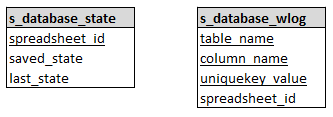
\includegraphics[width=0.5\textwidth]{resources/chapter-4-architect-db.png}
	    \caption{Diagram Struktur Tabel Penyimpanan Konfigurasi}
		\label{StructureDiagram}
	\end{figure}

	Tabel konfigurasi yang ditampilkan kepada pengguna akan berasal dari tabel s\_database\_state dan juga disimpan pada tabel tersebut. Kegunaan  s\_database\_wlog adalah mencatat pemetaan data kepada tabel konfigurasi sehingga saat tabel konfigurasi dihapus, data yang berasal dari tabel konfigurasi tersebut dapat juga dihapus.

	Modul-modul dan fitur dibuat diatas aplikasi EtherCalc, sehingga arsitektur aplikasi akan mengikuti arsitektur aplikasi EtherCalc yang telah dijelaskan pada Subbab \ref{TeknologiSpreadsheet}.

\section{Implementasi}
Implementasi dilakukan dengan membangun modul yang telah dijabarkan pada Subbab \ref{KebutuhanModul} dengan menggunakan bahasa Javascript, menyesuaikan dengan modul lain yang telah ada pada aplikasi EtherCalc. Pada bagian ini akan dijelaskan antarmuka dan modul-modul yang diimplementasikan.
	\subsection{Antarmuka}
	Antarmuka aplikasi pada Tugas Akhir ini mengikuti antarmuka yang telah ada sebelumnya pada aplikasi EtherCalc. Fitur baru yang ditambahkan akan menempati menu baru pada bagian atas antarmuka dengan nama `Data Collector`. Antarmuka awal dapat dilihat pada Gambar \ref{Antarmuka1}.

	\begin{figure}[htb]
	    \centering
	    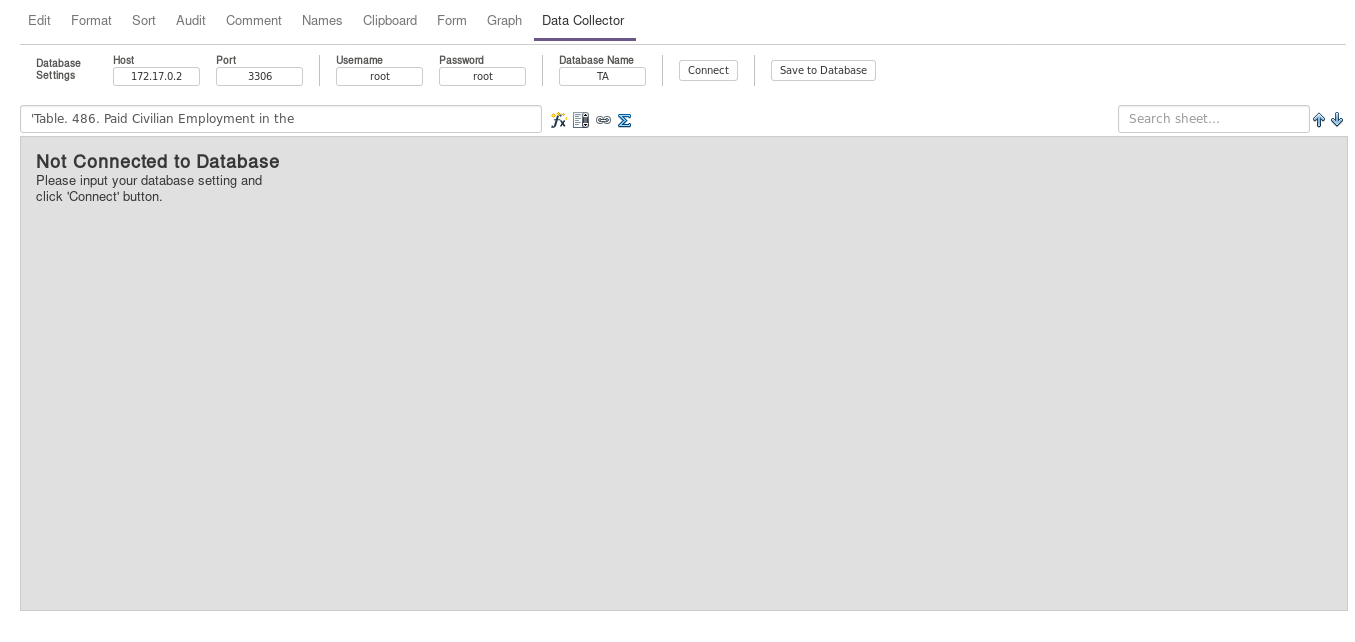
\includegraphics[width=1.0\textwidth]{resources/chapter-4-interface-1.png}
	    \caption{Antarmuka Awal}
		\label{Antarmuka1}
	\end{figure}

	Terdapat dua bagian utama pada antarmuka ini, yang pertama adalah area pengaturan basis data dimana pengguna bisa dapat mengatur koneksi ke basis data yang diinginkan. Yang kedua adalah area tempat tabel konfigurasi dapat ditambahkan dan dikurangi berdasarkan masukan pengguna. Pada bagian kiri area tabel konfigurasi, terdapat dua pilihan metode untuk membuat tabel konfigurasi yakni secara manual maupun otomatis. Kedua area ini dapat dilihat pada Gambar \ref{Antarmuka2}.

	\begin{figure}[htbp]
	    \centering
	    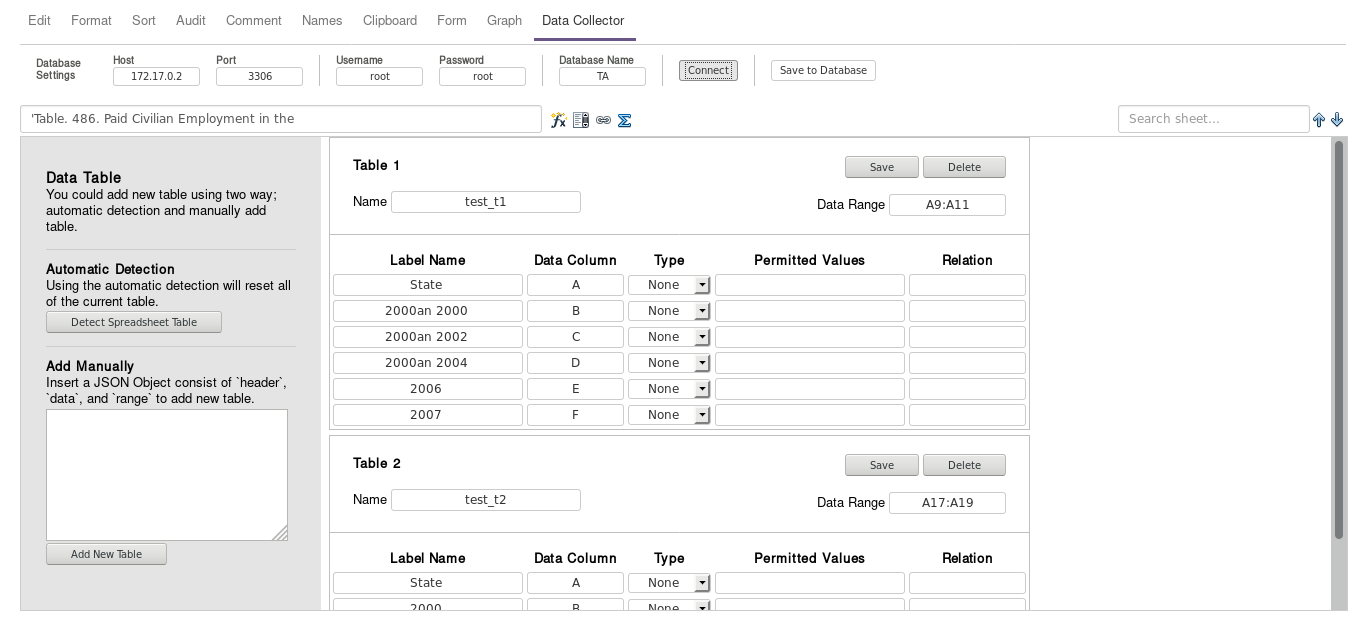
\includegraphics[width=1.0\textwidth]{resources/chapter-4-interface-2.png}
	    \caption{Antarmuka Tabel Konfigurasi}
		\label{Antarmuka2}
	\end{figure}

	Pada bagian tabel konfigurasi, pengguna dapat menentukan nama label, tipe data, nilai-nilai yang diizinkan, dan relasinya terhadap kumpulan sel lain untuk suatu kolom data. Selain itu, pengguna dapat juga mengubah nama tabel tujuan ke basis data serta menghapus tabel konfigurasi. Jika terjadi kesalahan pada saat validasi, pengguna akan diberikan pesan kesalahan dan diharapkan untuk memperbaiki data pada sel yang dianggap memiliki kesalahan. Interaksi ini dapat dilihat pada Gambar \ref{Antarmuka3}.

	\begin{figure}[htbp]
	    \centering
	    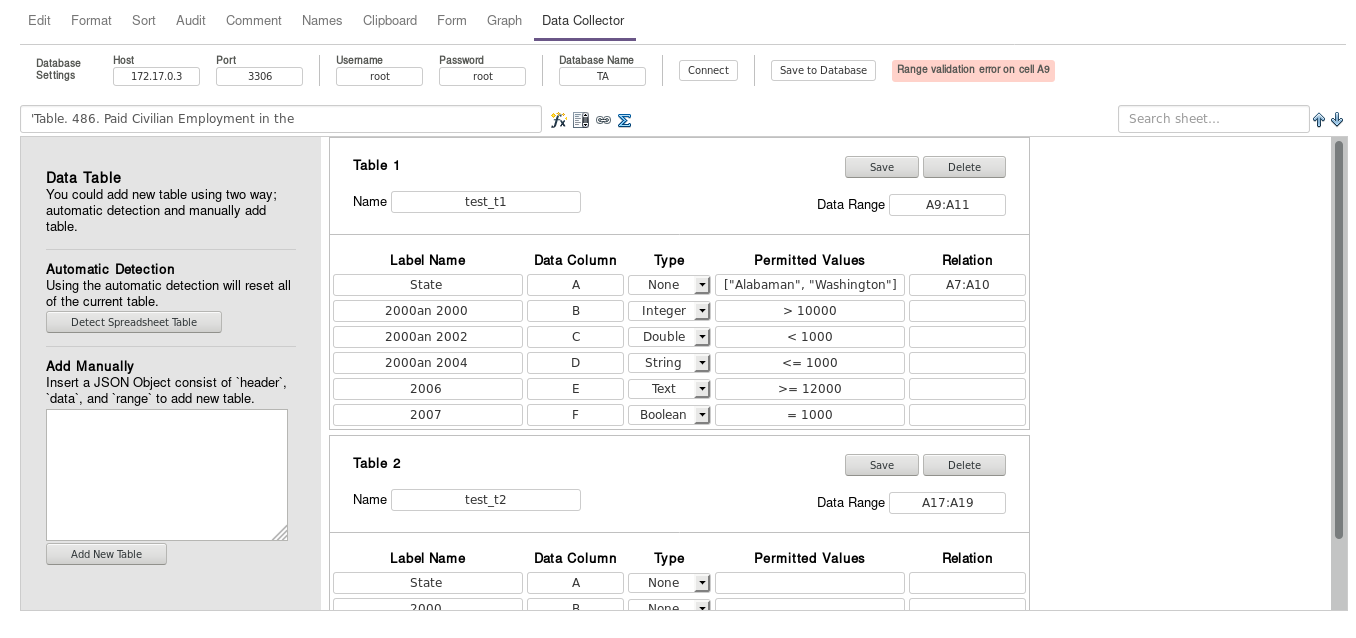
\includegraphics[width=1.0\textwidth]{resources/chapter-4-interface-3a.png}
	    \caption{Antarmuka Perubahan Tabel Konfigurasi}
		\label{Antarmuka3}
	\end{figure}
	
	\subsection{Modul Main}
	Modul \texttt{Main} tidak dibuat dari awal karena mengembangkan dari modul yang telah ada dari aplikasi EtherCalc. Modul ini yang menyediakan API agar dapat digunakan oleh aplikasi. Seluruh API ini akan dipanggil melalui modul \texttt{Player}. API yang ditambahkan pada Tugas Akhir ini adalah:
	\begin{enumerate}
		\item \texttt{POST /\_database/connect} \\
		Digunakan untuk melakukan pengecekan koneksi ke basis data. Parameter yang dibutuhkan adalah:
		\begin{itemize} 
			\item host: \textit{host} basis data.
			\item port: \textit{port} basis data.
			\item user: \textit{user} basis dat yang digunakan.
			\item password: \textit{password} untuk \textit{user} yang digunakan.
			\item database: nama \textit{database} yang digunakan.
		\end{itemize}
	
		\item \texttt{POST /\_database/state} \\
		Digunakan untuk melakukan penyimpanan \textit{state} tabel konfigurasi. Parameter yang dibutuhkan adalah:
		\begin{itemize} 
			\item tables: data tabel konfigurasi dalam bentuk JSON.
			\item setting: pengaturan koneksi ke basis data yang dipilih berupa JSON Object.
		\end{itemize}

		\item \texttt{POST /\_database/state/[spreadsheet\_id]} \\
		Digunakan untuk mendapatkan data \textit{state} tabel konfigurasi pada suatu \textit{spreadsheet}. Parameter yang dibutuhkan adalah::
		\begin{itemize}
			\item setting: pengaturan koneksi ke basis data yang dipilih berupa JSON Object.
		\end{itemize}

		\item \texttt{POST /\_database/create} \\
		Digunakan untuk melakukan penyimpanan data yang telah dikumpulkan sesuai dengan aturan pada tabel konfigurasi. Parameter yang dibutuhkan adalah:
		\begin{itemize} 
			\item table: data dari tabel konfigurasi yang telah diubah menjadi bentuk relasional dalam bentuk JSON.
			\item setting: pengaturan koneksi ke basis data yang dipilih berupa JSON Object.
		\end{itemize}
	
		\item \texttt{GET /\_framefinder/[spreadsheet\_id]/[start\_col]/[end\_col]\\/[start\_row]/[end\_row]} \\
		Digunakan untuk mendapatkan hasil pencarian label dan data diantara kolom dan baris tertentu.

		\item \texttt{GET /\_hierarchical/[spreadsheet\_id]} \\
		Digunakan untuk mendapatkan perkiraan kelompok sel yang merupakan suatu kesatuan tabel.	
	\end{enumerate}

	\subsection{Modul Player}
	Modul \texttt{player} merupakan modul yang menjembatani masukan pengguna dari yang berasal dari \textit{front-end} sehingga dapat diterima oleh modul yang berada di \textit{back-end}. Modul ini hanya terdiri dari satu kelas utama yakni kelas \texttt{player} yang berisi fungsi-fungsi yang dapat dipanggil oleh \textit{front-end} yang dapat dilihat pada Tabel \ref{FungsiModulPlayer}.

	\begin{small}
	\begin{longtable}{ | p{2cm} | p{10cm} | }
	    \caption{Fungsi pada Kelas \texttt{Player}}
	    \label{FungsiModulPlayer}\\ \hline
	    \centering\bfseries{Fungsi} & \centering\bfseries{Keterangan} \tabularnewline \hline
	    \endfirsthead
	    \hline
	    \centering\bfseries{Fungsi} & \centering\bfseries{Keterangan} \tabularnewline \hline
	    \endhead
	    refreshView & Melakukan pembaharuan tampilan sehingga menunjukkan tabel terbaru.\\ \hline
	    getDBSetting & Mengambil pengaturan basis data yang telah diberikan pengguna.\\ \hline
	    saveState & Menyimpan pengaturan yang telah dilakukan ke basis data.\\ \hline
	    loadState & Mengambil pengaturan yang pernah disimpan pada basis data.\\ \hline
	    saveConfig & Melakukan penyimpanan konfigurasi tabel yang dilakukan oleh pengguna. \\ \hline
	    deleteTable & Menghapus tabel konfigurasi yang dipilih.\\ \hline
	    addManual & Menambahkan tabel konfigurasi baru sesuai dengan masukan pengguna.\\ \hline
	    connect & Melakukan koneksi ke basis data yang dipilih. \\ \hline
	    save & Melakukan pemanggilan terhadap modul \texttt{table} dan melakukan penyimpanan ke basis data. \\ \hline
	    scan & Melakukan identifikasi tabel melalui pemanggilan modul \texttt{framefinder} yang selanjutnya akan menampilkan hasil identifikasi dan kolom perubahan konfigurasi yang dapat diisi pengguna. \\ \hline
	\end{longtable}
	\end{small}
	
	\subsection{Modul DB}
	Modul basis data digunakan sebagai antarmuka modul lain untuk melakukan operasi I/O basis data. Pada Tugas Akhir ini, basis data yang digunakan adalah MySQL. Modul ini hanya terdiri dari satu kelas utama yakni kelas \texttt{mysql}. Kelas ini memiliki tugas sebagai penghubung aplikasi ke basis data MySQL yang dipilih. Fungsi-fungsi yang terdapat pada kelas ini dapat dilihat pada Tabel \ref{FungsiModulDB}.

	\begin{small}
	\begin{longtable}{ | p{2cm} | p{10cm} | }
	    \caption{Fungsi pada Kelas \texttt{mysql}}
	    \label{FungsiModulDB}\\ \hline
	    \centering\bfseries{Fungsi} & \centering\bfseries{Keterangan} \tabularnewline \hline
	    \endfirsthead
	    \hline
	    \centering\bfseries{Fungsi} & \centering\bfseries{Keterangan} \tabularnewline \hline
	    \endhead
	    createTable & Fungsi yang digunakan untuk membuat Table tempat pengisian data.\\ \hline
	    isTableExists & Melakukan pengecekan ada atau tidaknya tabel tersebut pada basis data.\\ \hline
	    getColumns & Mendapatkan kolom-kolom yang ada pada suatu tabel.\\ \hline
	    selectData & Mendapatkan data sesuai dengan syarat yang diminta.\\ \hline
	    insertData & Memasukkan data ke dalam tabel yang dipilih.\\ \hline
	    deleteData & Menghapus data dari tabel.\\ \hline
	    updateData & Melakukan pembaharuan data dari tabel.\\ \hline
	    dropTable & Menghapus tabel yang dipilih.\\ \hline
	\end{longtable}
	\end{small}

	Tabel akan dibuat pada basis data yang ditentukan, setiap tabel merepresentasikan suatu tabel pada \textit{spreadsheet} yang ditentukan oleh pengguna. \textit{Header} yang didefinisikan oleh pengguna pada \textit{spreadsheet} akan dijadikan \textit{column} pada tabel basis data, tipe yang dibentuk mengikuti masukan pengguna. Tiap baris data yang ada dibawah \textit{header} pada \textit{spreadsheet} akan ditranslasikan menjadi bentuk relasional agar dapat dimasukan ke dalam tabel.
	
	\subsection{Modul Hierarchyfinder}
	Modul \texttt{hierarchyfinder} menggunakan algoritma \textit{hierarchical clustering} untuk dapat mengetahui mana yang merupakan suatu kesatuan tabel pada suatu \textit{sheet}. Modul ini dapat menentukan tabel-tabel yang terdapat pada suatu \textit{sheet} yang selanjutnya akan dilakukan identifikasi label oleh modul \texttt{framefinder}. Algoritma \textit{hierarchical clustering} yang digunakan menganggap setiap sel pada \textit{spreadsheet} merupakan suatu node. Sel-sel yang bersebelahan dengan sel tersebut akan dianggap tetangga sehingga memiliki jarak sama dengan 0. Sel yang digabungkan dengan sel lain akan dihitung sebagai satu \textit{node}. Aturan perhitungan jarak antar \textit{node} dapat dilihat pada kode di Kode \ref{KodeJarak}.\\

	\begin{lstlisting}[frame=single, basicstyle=\linespread{1}\scriptsize\listingsfont, captionpos=b, caption={Perhitungan Jarak \textit{Node}}, label=KodeJarak]
	# Fungsi cellDistance(v1, v2)
	# Parameter pada fungsi adalah v1 (node 1) dan v2 (node 2)
	t = new Table null, null
	colD = t.GetCellCol(v1[0]) - t.GetCellCol(v2[0])
	rowD = t.GetCellRow(v1[0]) - t.GetCellRow(v2[0])

	# Jika sel saling bertetangga tetapi bukan secara diagonal
	# Jika bertetangga, jarak kedua sel adalah 0
	if colD == 0
		if rowD == 1 or rowD == -1
			return 0
	if rowD == 0
		if colD == 1 or colD == -1
			return 0

	# Jika tidak, cek apakah sel bertetangga secara diagonal
	# Jika bertetangga, jarak kedua sel adalah 0
	leftTop = [[v1[1], v1[2]], [v2[1], v2[2]]]
	leftBot = [[v1[1], (v1[2] + v1[4])], [v2[1], (v2[2] + v2[4])]]
	righTop = [[(v1[1] + v1[3]), v1[2]], [(v2[1] + v2[3]), v2[2]]]
	righBot = [[(v1[1] + v1[3]), (v1[2] + v1[4])], [(v2[1] + v2[3]), (v2[2] + v2[4])]]

	if (leftTop[0][0] == righTop[1][0] and leftTop[0][1] == righTop[1][1])
		return 0
	if (leftBot[0][0] == righBot[1][0] and leftBot[0][1] == righBot[1][1])
		return 0

	if (leftTop[1][0] == righTop[0][0] and leftTop[1][1] == righTop[0][1])
		return 0
	if (leftBot[1][0] == righBot[0][0] and leftBot[1][1] == righBot[0][1])
		return 0

	if (leftTop[0][0] == leftBot[1][0] and leftTop[0][1] == leftBot[1][1])
		return 0
	if (righTop[0][0] == righBot[1][0] and righTop[0][1] == righBot[1][1])
		return 0

	if (leftTop[1][0] == leftBot[0][0] and leftTop[1][1] == leftBot[0][1])
		return 0
	if (righTop[1][0] == righBot[0][0] and righTop[1][1] == righBot[0][1])
		return 0

	# Jika tidak juga, hitung jarak menggunakan teknik Euclidian
	dist = Math.sqrt(Math.pow((v2[1] + (v2[3]/2)) - (v1[1] + (v1[3]/2)), 2) + Math.pow((v2[2] + (v2[4]/2)) - (v1[2] + (v1[4]/2)), 2));
	return dist
	\end{lstlisting}

	Hasil dari pengelompokan ini berupa kelompok-kelompok tabel pada \textit{spreadsheet}. Setiap tabel yang teridentifikasi selanjutnya akan dicari bagian \textit{header} dan \textit{label} menggunakan modul \texttt{framefinder}.

	\subsection{Modul Framefinder}
	Modul \texttt{framefinder} melakukan pengidentifikasian terhadap tabel yang ada sehingga dapat diketahui baris yang merupakan \textit{header} dan \textit{data}. Implementasi modul ini dilakukan dengan mengikuti implementasi yang dilakukan pada penelitian yang dilakukan oleh Chen \citep{Chen2013}. Modul ini terdiri dari 5 kelas yang dapat dilihat pada Tabel \ref{KelasModulFF}.

	\begin{small}
	\begin{longtable}{ | p{3cm} | p{10cm} | }
	    \caption{Kelas pada Modul \texttt{FrameFinder}}
	    \label{KelasModulFF}\\ \hline
	    \centering\bfseries{Nama Kelas} & \centering\bfseries{Keterangan} \tabularnewline \hline
	    \endfirsthead
	    \hline
	    \centering\bfseries{Nama Kelas} & \centering\bfseries{Keterangan} \tabularnewline \hline
	    \endhead
	    LoadSheet & Kelas ini berfungsi sebagai kelas yang melakukan pengambilan data dan konversi sel dan \textit{sheet} pada \textit{spreadsheet} ke dalam bentuk kelas-kelas yang ada pada modul ini.\\ \hline
	    MySheet & Merupakan kelas bentukan yang merepresentasikan \textit{sheet} pada \textit{spreadsheet} yang dipilih.\\ \hline
	    MyCell & Merupakan kelas untuk merepresentasikan \textit{properties} yang ada pada sel pada \textit{sheet} yang dipilih.\\ \hline
	    FeatureSheetRow & Melakukan ekstraksi fitur-fitur yang terdapat pada suatu \textit{sheet} pada \textit{spreadsheet}.\\ \hline
	    PredictSheetRows & Kelas ini digunakan untuk menghasilkan file dalam format yang dapat dibaca oleh algoritma Conditional Random Field (CRF) dari fitur-fitur yang telah diekstraksi pada \textit{sheet}.\\ \hline
	\end{longtable}
	\end{small}

	\subsubsection{Kelas LoadSheet}
	Kelas ini melakukan pengambilan data pada \textit{spreadsheet} dengan cara membaca file \textit{spreadsheet} dan membentuk representasi kelas yang dibutuhkan. Kelas ini memiliki satu atribut utama yakni cmysheet yang merupakan kelas MySheet. Fungsi-fungsi yang terdapat pada kelas ini dapat dilihat pada Tabel \ref{FungsiLoadSheet}.

	\begin{small}
	\begin{longtable}{ | p{4cm} | p{9cm} | }
	    \caption{Fungsi pada Kelas LoadSheet}
	    \label{FungsiLoadSheet}\\ \hline
	    \centering\bfseries{Nama Fungsi} & \centering\bfseries{Keterangan} \tabularnewline \hline
	    \endfirsthead
	    \hline
	    \centering\bfseries{Nama Fungsi} & \centering\bfseries{Keterangan} \tabularnewline \hline
	    \endhead
	    loadSheetDict & Fungsi ini merupakan fungsi utama yang bertugas untuk membuat representasi \textit{spreadsheet} yang diterima ke dalam kelas MySheet.\\ \hline
	    getValueType & Untuk mendapatkan tipe representasi data yang diberikan oleh \textit{spreadsheet}. Contoh: tanggal, nominal uang, desimal, dan lain-lain.\\ \hline
	    getDataType & Untuk mendapatkan tipe data primitif pada suatu sel.\\ \hline
	    featureIndentation & Digunakan untuk mengecek keberadaan \textit{property} \textit{indentation} pada sel.\\ \hline
	    featureAlignStyle & Digunakan untuk mengecek keberadaan \textit{property} \textit{align} pada sel\\ \hline
	    featureFontBold & Digunakan untuk mengecek keberadaan \textit{property} \textit{bold} pada sel\\ \hline
	    featureFontHeight & Digunakan untuk mengecek keberadaan \textit{property} \textit{height} pada sel\\ \hline
	    featureFontUnderline & Digunakan untuk mengecek keberadaan \textit{property} \textit{underline} pada sel\\ \hline
	    featureFontItalic & Digunakan untuk mengecek keberadaan \textit{property} \textit{italic} pada sel\\ \hline
	    featureFontBgcolor & Digunakan untuk mengecek keberadaan \textit{property} \textit{background color} pada sel\\ \hline
	    featureBorderStyle & Digunakan untuk mengecek keberadaan \textit{property} \textit{border} pada sel.\\ \hline
	\end{longtable}
	\end{small}

	\subsubsection{Kelas MySheet}
	Kelas MySheet merupakan kelas yang merepresentasikan \textit{sheet} pada \textit{spreadsheet} yang dipilih. Kelas ini memiliki 4 atribut yang dapat dilihat pada Tabel \ref{AtributMySheet}.

	\begin{small}
	\begin{longtable}{ | p{3cm} | p{8cm} | }
	    \caption{Atribut pada Kelas MySheet}
	    \label{AtributMySheet}\\ \hline
	    \centering\bfseries{Nama Atribut} & \centering\bfseries{Keterangan} \tabularnewline \hline
	    \endfirsthead
	    \hline
	    \centering\bfseries{Nama Atribut} & \centering\bfseries{Keterangan} \tabularnewline \hline
	    \endhead
	    sheetdict & Merupakan representasi kumpulan sel-sel pada suatu \textit{sheet}. Tiap sel direpresentasikan dalam bentuk kelas MyCell.\\ \hline
	    mergerowdict & Merupakan kumpulan sel-sel yang digabungkan.\\ \hline
	    maxcolnum & Nilai kolom terbesar pada sel.\\ \hline
	    maxrownum & Nilai baris terbesar pada sel.\\ \hline
	\end{longtable}
	\end{small}

	Pada kelas ini terdapat 3 fungsi yang dapat dilihat pada Tabel \ref{FungsiMySheet}.

	\begin{small}
	\begin{longtable}{ | p{4cm} | p{9cm} | }
	    \caption{Fungsi pada Kelas MySheet}
	    \label{FungsiMySheet}\\ \hline
	    \centering\bfseries{Nama Fungsi} & \centering\bfseries{Keterangan} \tabularnewline \hline
	    \endfirsthead
	    \hline
	    \centering\bfseries{Nama Fungsi} & \centering\bfseries{Keterangan} \tabularnewline \hline
	    \endhead
	    getCellsArray & Digunakan untuk mendapatkan seluruh refresentasi sel pada kelas ini dalam bentuk \textit{array}.\\ \hline
	    addMergeCell & Digunakan pada saat terdapat sel yang digabungkan. Sel tersebut akan dimasukkan ke dalam daftar \textit{merged cells}.\\ \hline
	    insertCell & Menambahkan sel ke dalam kelas ini. Sel yang ditambahkan akan direpresentasikan dalam bentuk kelas MyCell.\\ \hline
	\end{longtable}
	\end{small}

	\subsubsection{Kelas MyCell}
	Kelas MyCell merupakan kelas yang merepresentasikan sel pada suatu \textit{sheet}. Kelas ini memiliki 17 atribut yang dapat dilihat pada Tabel \ref{AtributMyCell}.

	\begin{small}
	\begin{longtable}{ | p{3cm} | p{8cm} | }
	    \caption{Atribut pada Kelas MyCell}
	    \label{AtributMyCell}\\ \hline
	    \centering\bfseries{Nama Atribut} & \centering\bfseries{Keterangan} \tabularnewline \hline
	    \endfirsthead
	    \hline
	    \centering\bfseries{Nama Atribut} & \centering\bfseries{Keterangan} \tabularnewline \hline
	    \endhead
	    x & Merupakan letak sel pada koordinat X.\\ \hline
	    y & Merupakan letak sel pada koordinat Y. \\ \hline
	    w & Nilai lebar sel.\\ \hline
	    h & Nilai tinggi sel.\\ \hline
	    cstr & Isi sel dalam bentuk \textit{string}.\\ \hline
	    mtype & Tipe konten yang ada di dalam sel.\\ \hline
	    indents & Nilai indentasi jika terdapat indentasi pada konten.\\ \hline
	    centeralign & Bernilai \textit{true} atau \textit{false} bergantung pada \textit{align} sel merupakan rata tengah atau tidak.\\ \hline
	    leftalign & Bernilai \textit{true} atau \textit{false} bergantung pada \textit{align} sel merupakan rata kiri atau tidak.\\ \hline
	    rightalign & Bernilai \textit{true} atau \textit{false} bergantung pada \textit{align} sel merupakan rata kanan atau tidak.\\ \hline
	    bottomborder & Bernilai \textit{true} atau \textit{false} bergantung pada \textit{property} \textit{bottom border} ada atau tidak.\\ \hline
	    upperborder & Bernilai \textit{true} atau \textit{false} bergantung pada \textit{property} \textit{upper border} ada atau tidak.\\ \hline
	    leftborder & Bernilai \textit{true} atau \textit{false} bergantung pada \textit{property} \textit{left border} ada atau tidak.\\ \hline
	    rightborder & Bernilai \textit{true} atau \textit{false} bergantung pada \textit{property} \textit{right border} ada atau tidak.\\ \hline
	    bold & Bernilai \textit{true} atau \textit{false} bergantung pada \textit{property} \textit{bold} ada atau tidak.\\ \hline
	    italic & Bernilai \textit{true} atau \textit{false} bergantung pada \textit{property} \textit{italic} ada atau tidak.\\ \hline
	    underline & Bernilai \textit{true} atau \textit{false} bergantung pada \textit{property} \textit{underline} ada atau tidak.\\ \hline
	\end{longtable}
	\end{small}

	% Pada kelas ini terdapat 3 fungsi yang dapat dilihat pada Tabel \ref{FungsiMyCell}.

	% \begin{small}
	% \begin{longtable}{ | p{4cm} | p{9cm} | }
	%     \caption{Fungsi pada Kelas MyCell}
	%     \label{FungsiMyCell}\\ \hline
	%     \centering\bfseries{Nama Fungsi} & \centering\bfseries{Keterangan} \tabularnewline \hline
	%     \endfirsthead
	%     \hline
	%     \centering\bfseries{Nama Fungsi} & \centering\bfseries{Keterangan} \tabularnewline \hline
	%     \endhead
	%     writestrAlignstyle & Mendapatkan representasi \textit{string} untuk \textit{align} pada sel. Digunakan pada saat penulisan ke dalam file untuk dibaca pada algoritma CRF.\\ \hline
	%     writestrBorderstyle & Mendapatkan representasi \textit{string} untuk \textit{border} pada sel. Digunakan pada saat penulisan ke dalam file untuk dibaca pada algoritma CRF.\\ \hline
	%     getIndents & Digunakan untuk menentukan nilai atribut indentasi dengan menghitung seberapa dalam indentasi pada konten.\\ \hline
	% \end{longtable}
	% \end{small}

	\subsubsection{Kelas FeatureSheetRow}
	Kelas ini bertugas untuk melakukan ekstraksi fitur pada tiap baris sel yang telah dikumpulkan dari \textit{spreadsheet}. Fitur-fitur yang diambil untuk setiap barisnya dapat dilihat pada Tabel \ref{FiturEkstraksi}.

	\begin{small}
	\begin{longtable}{ | p{10cm} | }
	    \caption{Fitur yang Diambil dari Sel}
	    \label{FiturEkstraksi}\\ \hline
	    \centering\bfseries{Fitur} \tabularnewline \hline
	    \endfirsthead
	    \hline
	    \centering\bfseries{Fitur} \tabularnewline \hline
	    \endhead
	    Baris memiliki sel yang digabung \\ \hline
	    Sel pada baris mencapai kolom paling kanan \\ \hline
	    Sel pada baris mencapai kolom paling kiri \\ \hline
	    Baris hanya memiliki 1 kolom \\ \hline
	    Baris memiliki sel rata tengah \\ \hline
	    Baris memiliki sel rata kiri \\ \hline
	    Baris memiliki sel yang ditebalkan (\textit{bold}) \\ \hline
	    Baris memiliki sel berindentasi \\ \hline
	    Baris memiliki sel berisi kata `Table` \\ \hline
	    Baris memiliki sel berisi kata berawalan tanda baca \\ \hline
	    Baris memiliki sel dengan presentase angka tinggi \\ \hline
	    Baris memiliki sel berisi huruf besar seluruhnya \\ \hline
	    Baris memiliki sel berisi kata dengan awal huruf besar \\ \hline
	    Baris memiliki sel berisi kata dengan awal huruf kecil \\ \hline
	    Baris memiliki persentase sel memiliki isi tinggi \\ \hline
	    Baris memiliki persentase sel memiliki isi berupa kata tinggi \\ \hline
	    Baris memiliki sel berisi karakter spesial \\ \hline
	    Baris memiliki sel berisi karakter titik koma \\ \hline
	    Baris memiliki jumlah sel berisi tahun tinggi \\ \hline
	    Baris memiliki persentase sel berisi tahun tinggi \\ \hline
	    Baris memiliki jumlah sel berisi kata dengan huruf yang banyak tinggi \\ \hline
	\end{longtable}
	\end{small}

	Fitur-fitur diatas mengikuti fitur yang didefinisikan pada penelitian yang dilakukan oleh Chen \citep{Chen2013}. Fitur-fitur ini akan digunakan dalam perhitungan algoritma CRF.

	\subsubsection{Kelas PredictSheetRows}
	Kelas PredictSheetRows memiliki tugas untuk melakukan konversi fitur-fitur yang telah didapatkan pada kelas FeatureSheetRow menjadi bentuk file teks yang dapat dibaca oleh program CRFPP yang akan menjalankan algoritma CRF pada file tersebut. Contoh file yang dihasilkan oleh kelas ini dapat dilihat pada Kode \ref{KodeFile}.\\

	\begin{lstlisting}[frame=single, basicstyle=\linespread{1}\scriptsize\listingsfont, captionpos=b, caption={File Berisikan Fitur Tiap Baris}, label=KodeFile]
	DeadlineTA.xls____Sheet1____1 1 0 1 0 0 1 0 1 0 0 0 0 0 0 1 0 1 1 0 0 0 0 0 Header
	DeadlineTA.xls____Sheet1____2 0 1 1 0 0 1 0 0 0 0 0 1 0 0 1 0 1 1 0 0 0 0 0 Data
	DeadlineTA.xls____Sheet1____3 0 1 1 0 0 1 0 0 0 0 0 1 0 0 1 0 0 0 0 0 0 0 0 Data
	DeadlineTA.xls____Sheet1____4 0 1 1 0 0 1 0 0 0 0 0 1 0 0 1 0 0 0 0 0 0 0 0 Data
	DeadlineTA.xls____Sheet1____5 0 1 1 0 0 1 0 0 0 0 0 1 0 0 1 0 0 1 0 0 0 0 0 Data
	\end{lstlisting}

	File tersebut ditulis dalam format \texttt{namafile\_namasheet\_bariske [fitur-fitur pada baris] label}. File ini yang akan diolah oleh algoritma dan digunakan untuk memprediksi label dari setiap baris tersebut. Algoritma yang digunakan adalah Conditional Random Field dan menggunakan aplikasi CRFPP yang berjalan eksternal diluar kelas ini untuk membaca file, membaca model, serta memprediski label.

	\subsection{Modul Table}
	Modul \texttt{table} memiliki tugas untuk mengelola tampilan dan isi tabel konfigurasi, melakukan validasi data masukan, dan membuat representasi relasional yang dapat diterima oleh basis data. Modul \texttt{table} hanya memiliki satu kelas yakni kelas \texttt{table}. Kelas ini memiliki 8 atribut yang dapat dilihat pada Tabel \ref{AtributTable}.

	\begin{small}
	\begin{longtable}{ | p{3cm} | p{8cm} | }
	    \caption{Atribut pada Kelas Table}
	    \label{AtributTable}\\ \hline
	    \centering\bfseries{Nama Atribut} & \centering\bfseries{Keterangan} \tabularnewline \hline
	    \endfirsthead
	    \hline
	    \centering\bfseries{Nama Atribut} & \centering\bfseries{Keterangan} \tabularnewline \hline
	    \endhead
	    sheet & Berisikan data untuk masing-masing sel pada suatu \textit{sheet}.\\ \hline
	    rows & Representasi tabel yang berisikan; nama \textit{header}, kolom data, dan aturan-aturan validasi.\\ \hline
	    range & \textit{Range} sel data pada tabel.\\ \hline
	    title & Kumpulan baris yang diidentifikasi sebagai \textit{title} oleh pengenalan otomatis.\\ \hline
	    footnote & Kumpulan baris yang diidentifikasi sebagai \textit{footnote} oleh pengenalan otomatis.\\ \hline
	    header & Kumpulan baris yang diidentifikasi sebagai \textit{header} oleh pengenalan otomatis.\\ \hline
	    data & Kumpulan baris yang diidentifikasi sebagai \textit{data} oleh pengenalan otomatis.\\ \hline
	    name & Nama tabel yang akan dijadikan nama tabel pada basis data.\\ \hline
	\end{longtable}
	\end{small}

	Pada kelas ini terdapat 6 fungsi yang dapat dilihat pada Tabel \ref{FungsiMySheet}.

	\begin{small}
	\begin{longtable}{ | p{4cm} | p{9cm} | }
	    \caption{Fungsi pada Kelas LoadSheet}
	    \label{FungsiLoadSheet}\\ \hline
	    \centering\bfseries{Nama Fungsi} & \centering\bfseries{Keterangan} \tabularnewline \hline
	    \endfirsthead
	    \hline
	    \centering\bfseries{Nama Fungsi} & \centering\bfseries{Keterangan} \tabularnewline \hline
	    \endhead
	    ParseData & Melakukan \textit{parse} terhadap data dari \textit{spreadsheet} menjadi bentuk objek tabel. \\ \hline
		TupleSerializeWithChecker & Digunakan untuk mengubah struktur tabel menjadi tabel relasional dan melakukan validasi data masukan sesuai dengan aturan yang diminta pengguna.\\ \hline
		Serialize & Mengubah objek tabel menjadi JSON.\\ \hline
		Deserialize & Mengubah JSON menjadi objek tabel.\\ \hline
		GetHTMLForm & Menghasilkan bentuk HTML dari objek tabel agar dapat ditampilkan pada antarmuka.\\ \hline
	\end{longtable}
	\end{small}

	Modul ini berinteraksi langsung dengan modul \texttt{player} pada saat akan melakukan penyimpanan \textit{state} tabel konfigurasi dan menampilkan tabel konfigurasi pada \textit{front-end}. Selain itu, modul ini juga berhubungan dengan modul \texttt{mysql} pada saat melakukan penyimpanan.

\section{Pengujian}
Pengujian dilakukan hanya kepada fitur yang di buat pada Tugas Akhir ini dan tidak kepada aplikasi EtherCalc secara keseluruhan. Pada subbab ini akan dibahas kasus-kasus yang diuji dan hasil dari pengujian tersebut.

	\subsection{Tujuan Pengujian}
	Pada fitur yang dibangun pada Tugas Akhir ini, pengujian yang dilakukan mempunyai tujuan yaitu:
	\begin{enumerate}
		\item Memastikan bahwa fitur yang diimplementasi dapat berjalan dengan baik. Pengujian yang dilakukan akan dikaitkan pada kasus-kasus penggunaan yang dapat terjadi. Dari pengujian akan dilihat kesesuaian hasil sesungguhnya dengan hasil yang diinginkan.
		\item Mencatat waktu eksekusi yang dibutuhkan untuk fitur-fitur yang ditambahkan.
	\end{enumerate}

	\subsection{Lingkungan Pengujian}
	Pengujian dilakukan pada komputer dengan spesifikasi pada Tabel \ref{LingPengujian}.

	\begin{small}
	\begin{longtable}{ | p{3cm} | p{9cm} | }
	    \caption{Spesifikasi Lingkungan Pengujian}
	    \label{LingPengujian}\\ \hline
	    \centering\bfseries{Komponen} & \centering\bfseries{Keterangan} \tabularnewline \hline
	    \endfirsthead
	    \hline
	    \centering\bfseries{Komponen} & \centering\bfseries{Keterangan} \tabularnewline \hline
	    \endhead
		Prosesor & AMD A8-4500M APU with Radeon(tm) HD Graphics 1.90GHz\\ \hline
		Memori Fisik & 12 GB\\ \hline
		\textit{Storage} & 50 GB\\ \hline
		Sistem Operasi & Arch Linux 64-bit\\ \hline
		Docker version & 1.13.1\\ \hline
		\textit{Web browser} & Mozilla Firefox 51.0.1\\ \hline
	\end{longtable}
	\end{small}

	\subsection{Eksekusi Pengujian} \label{skenarioujian}
	Kasus pengujian disesuaikan dengan kebutuhan fungsional dan non-fungsional yang sudah dijelaskan pada Subbab \ref{PerancanganPL}. Setiap kasus uji diberi kode TC-XX dengan XX adalah nomor kasus uji. Daftar kasus uji dapat diperhatikan pada Tabel \ref{KasusUjiFA}.

	\begin{small}
	\begin{longtable}{ | p{2cm} | p{8cm} | p{3cm} | }
	    \caption{Kasus Uji Fitur Aplikasi}
	    \label{KasusUjiFA}\\ \hline
	    \centering\bfseries{ID} & \centering\bfseries{Tujuan} & \centering\bfseries{ID kebutuhan terkait} \tabularnewline \hline
	    \endfirsthead
	    \hline
	    \centering\bfseries{ID} & \centering\bfseries{Tujuan} & \centering\bfseries{ID kebutuhan terkait} \tabularnewline \hline
	    \endhead
		TC-01 & Terkoneksi ke basis data MySQL yang dipilih pengguna dan dapat menggunakan basis data tersebut& FR-01, FR-02 \\ \hline
		TC-02 & Mendeteksi label dan data secara otomatis pada \textit{spreadsheet} & FR-04, FR-05 \\ \hline
		TC-03 & Menambahkan tabel konfigurasi secara manual sesuai dengan masukan pengguna & FR-04 \\ \hline
		TC-04 & Pengguna dapat mengubah atribut yang ada pada tabel konfigurasi & FR-06 \\ \hline
		TC-05 & Data dapat dimasukkan ke basis data sesuai dengan tabel konfigurasi & FR-03, FR-09, NF-01 \\ \hline
		TC-06 & Data yang dimasukkan ke basis data berhasil divalidasi sesuai aturan pengguna & FR-07, FR-08, FR-09, NF-01 \\ \hline	
		TC-07 & Pencatatan \textit{response time} pada fitur yang ditambahkan & FN-03 \\ \hline
	\end{longtable}
	\end{small}

	\subsection{Hasil Pengujian}
	Hasil pengujian dikaitkan dengan ID skenario pengujian yang berkaitan langsung dengan kasus uji yang telah didefinisikan pada Bab \ref{skenarioujian}. Tiap hasil pengujian mempunyai ID skenario terkait, ekspektasi, hasil uji yang dilakukan, dan diterima atau tidaknya hasil pengujian. Hasil pengujian merupakan hasil pelaksanaan skenario yang sudah dibuat dan dapat diperhatikan pada Lampiran A.

    \chapter{Kesimpulan dan Saran}
Bab ini berisi hal-hal yang dapat disimpulkan dari pelaksanaan Tugas Akhir ini. Bab ini juga mencakup saran untuk pengembangan Tugas Akhir ini di masa mendatang.

\section{Kesimpulan}
Berdasarkan hasil pengembangan kakas pengumpulan data menggunakan \textit{spreadsheet} yang telah dilakukan. Berikut adalah kesimpulan yang diperoleh.
\begin{enumerate}
	\item Telah berhasil dilakukan penambahan fitur pada aplikasi EtherCalc yang dapat melakukan pengumpulan data ke dalam bentuk basis data.
	% \item Konflik pada kolaborasi dapat ditangani dengan baik oleh sistem pada EtherCalc sehingga penanganan konflik tidak perlu dibuat kembali.
	\item Data yang akan dimasukkan ke basis data penyimpanan berhasil divalidasi menggunakan fitur yang dibuat dengan tiga tipe validasi yakni tipe data, domain data, dan relasi data.
	\item Identifikasi tabel pada suatu \textit{sheet} dapat dilakukan dengan menggunakan algoritma kNN dengan mencari kedekatan antar sel. Identifikasi label suatu baris pada tabel dapat dilakukan dengan teknik \textit{frame finder} dengan membagi label menjadi empat jenis yakni \textit{title}, \textit{data}, \textit{header}, dan \textit{footer}. Jika teknik \textit{frame finder} tidak berhasil menemukan label dan data, maka pengguna dapat memasukkan \textit{metadata table} secara manual dan mengubahnya sesuai dengan keinginan pengguna.
	\item Penggabungan data antar \textit{spreadsheet} dapat dilakukan dengan fitur yang dibuat dan dapat digabungkan secara horizontal, vertikal, maupun gabungan keduanya. Data pada \textit{spreadsheet} berhasil dimasukkan ke dalam basis data yang ditentukan sesuai dengan \textit{metadata table} yang telah dibuat pengguna maupun hasil pencarian otomatis dari algoritma \textit{frame finder}.
	\item Alur kerja pengumpulan data berubah sehingga dapat diusulkan alur kerja baru dimana \textit{versioning} dilakukan oleh aplikasi EtherCalc karena seluruh data berada pada satu tempat menggunakan mekanisme penyimpanan oleh EtherCalc. Pada saat pengumpulan data dari berbagai \textit{spreadsheet} dapat dilakukan menggunakan aplikasi yang sama yakni EtherCalc, sehingga pada alur kerja yang diusulkan, pengumpulan data tidak memerlukan bantuan aplikasi lain ataupun manual. Hasil akhir dari pengumpulan data merupakan data pada basis data sehingga data mudah diolah, ditampilkan, maupun diubah menggunakan banyak aplikasi yang tersedia.
\end{enumerate}

\section{Saran}
Saran yang dapat diberikan untuk pengembangan di masa mendatang adalah sebagai berikut:
\begin{enumerate}
	\item Pada pembangunan selanjutnya dapat ditambahkan penanganan kasus penggunaan \textit{spreadsheet} selain \textit{data frame} dan relasi.
	\item Penambahan data pembelajaran untuk identifikasi label baris dapat dilakukan sehingga akan memperbaiki hasil identifikasi otomatis. Pada pengembangan selanjutnya dapat ditambahkan \textit{feedback} dari pengguna sebagai data pembelajaran.
	\item Menambahkan fungsionalitas yakni memperbolehkan kolom \textit{key} yang tidak hanya satu pada \textit{metadata table}.
	\item Pengembangan fitur validasi, contohnya adalah menambahkan jenis validasi contohnya validasi masukan berbentuk formula. Di samping itu, dapat ditambahkan jenis validasi pada validasi tipe seperti tipe tanggal. Dapat juga penambahan fitur pada validasi domain seperti atribut yang dapat menerima tidak hanya satu aturan validasi domain.
	\item Penanganan jenis tabel dengan \textit{header} yang berada di kiri dan kanan data mungkin dapat dikembangkan menggunakan teknik \textit{transpose}.

\end{enumerate}
    %----------------------------------------------------------------%

    % Daftar pustaka
    % Bibliography to Daftar Pustaka
    \renewcommand{\bibname}{Daftar Pustaka}
    \cleardoublepage
    \phantomsection
    \addcontentsline{toc}{chapter}{DAFTAR PUSTAKA}
    %\printbibliography
    \bibliography{references}
    \bibliographystyle{apa}

    % Index
    \appendix

    \cleardoublepage
    \phantomsection
    %\part*{Lampiran}
    %\addcontentsline{toc}{part}{LAMPIRAN}

    %\chapter{Lampiran A. Detail Implementasi}

\begin{small}
\begin{longtable}{ | p{2cm} | p{10cm} | }
    \caption{Fungsi pada Kelas \texttt{player}}
    \label{FungsiModulPlayer}\\ \hline
    \centering\bfseries{Fungsi} & \centering\bfseries{Deskripsi} \tabularnewline \hline
    \endfirsthead
    \hline
    \centering\bfseries{Fungsi} & \centering\bfseries{Deskripsi} \tabularnewline \hline
    \endhead
    refreshView & Melakukan pembaharuan tampilan sehingga menunjukkan tabel terbaru.\\ \hline
    getDBSetting & Mengambil pengaturan basis data yang telah diberikan pengguna.\\ \hline
    saveState & Menyimpan pengaturan yang telah dilakukan ke basis data.\\ \hline
    loadState & Mengambil pengaturan yang pernah disimpan pada basis data.\\ \hline
    saveConfig & Melakukan penyimpanan konfigurasi tabel yang dilakukan oleh pengguna. \\ \hline
    deleteTable & Menghapus \textit{metadata table} yang dipilih.\\ \hline
    addManual & Menambahkan \textit{metadata table} baru sesuai dengan masukan pengguna.\\ \hline
    connect & Melakukan koneksi ke basis data yang dipilih. \\ \hline
    save & Melakukan pemanggilan terhadap modul \texttt{table} dan melakukan penyimpanan ke basis data. \\ \hline
    scan & Melakukan identifikasi tabel melalui pemanggilan modul \texttt{framefinder} yang selanjutnya akan menampilkan hasil identifikasi dan kolom perubahan konfigurasi yang dapat diisi pengguna. \\ \hline
\end{longtable}
\end{small}

\begin{small}
\begin{longtable}{ | p{2cm} | p{10cm} | }
    \caption{Fungsi pada Kelas \texttt{mysql}}
    \label{FungsiModulDB}\\ \hline
    \centering\bfseries{Fungsi} & \centering\bfseries{Deskripsi} \tabularnewline \hline
    \endfirsthead
    \hline
    \centering\bfseries{Fungsi} & \centering\bfseries{Deskripsi} \tabularnewline \hline
    \endhead
    createTable & Fungsi yang digunakan untuk membuat Table tempat pengisian data.\\ \hline
    isTableExists & Melakukan pengecekan ada atau tidaknya tabel tersebut pada basis data.\\ \hline
    getColumns & Mendapatkan kolom-kolom yang ada pada suatu tabel.\\ \hline
    selectData & Mendapatkan data sesuai dengan syarat yang diminta.\\ \hline
    insertData & Memasukkan data ke dalam tabel yang dipilih.\\ \hline
    deleteData & Menghapus data dari tabel.\\ \hline
    updateData & Melakukan pembaharuan data dari tabel.\\ \hline
    dropTable & Menghapus tabel yang dipilih.\\ \hline
\end{longtable}
\end{small}

\begin{small}
\begin{longtable}{ | p{3cm} | p{10cm} | }
    \caption{Kelas pada Modul \texttt{FrameFinder}}
    \label{KelasModulFF}\\ \hline
    \centering\bfseries{Nama Kelas} & \centering\bfseries{Deskripsi} \tabularnewline \hline
    \endfirsthead
    \hline
    \centering\bfseries{Nama Kelas} & \centering\bfseries{Deskripsi} \tabularnewline \hline
    \endhead
    LoadSheet & Kelas ini berfungsi sebagai kelas yang melakukan pengambilan data dan konversi sel dan \textit{sheet} pada \textit{spreadsheet} ke dalam bentuk kelas-kelas yang ada pada modul ini.\\ \hline
    MySheet & Merupakan kelas bentukan yang merepresentasikan \textit{sheet} pada \textit{spreadsheet} yang dipilih.\\ \hline
    MyCell & Merupakan kelas untuk merepresentasikan \textit{properties} yang ada pada sel pada \textit{sheet} yang dipilih.\\ \hline
    FeatureSheetRow & Melakukan ekstraksi fitur-fitur yang terdapat pada suatu \textit{sheet} pada \textit{spreadsheet}.\\ \hline
    PredictSheetRows & Kelas ini digunakan untuk menghasilkan file dalam format yang dapat dibaca oleh algoritma Conditional Random Field (CRF) dari fitur-fitur yang telah diekstraksi pada \textit{sheet}.\\ \hline
\end{longtable}
\end{small}

\begin{small}
\begin{longtable}{ | p{4cm} | p{9cm} | }
    \caption{Fungsi pada Kelas LoadSheet}
    \label{FungsiLoadSheet}\\ \hline
    \centering\bfseries{Nama Fungsi} & \centering\bfseries{Deskripsi} \tabularnewline \hline
    \endfirsthead
    \hline
    \centering\bfseries{Nama Fungsi} & \centering\bfseries{Deskripsi} \tabularnewline \hline
    \endhead
    loadSheetDict & Fungsi ini merupakan fungsi utama yang bertugas untuk membuat representasi \textit{spreadsheet} yang diterima ke dalam kelas MySheet.\\ \hline
    getValueType & Untuk mendapatkan tipe representasi data yang diberikan oleh \textit{spreadsheet}. Contoh: tanggal, nominal uang, desimal, dan lain-lain.\\ \hline
    getDataType & Untuk mendapatkan tipe data primitif pada suatu sel.\\ \hline
    featureIndentation & Digunakan untuk mengecek keberadaan \textit{property} \textit{indentation} pada sel.\\ \hline
    featureAlignStyle & Digunakan untuk mengecek keberadaan \textit{property} \textit{align} pada sel\\ \hline
    featureFontBold & Digunakan untuk mengecek keberadaan \textit{property} \textit{bold} pada sel\\ \hline
    featureFontHeight & Digunakan untuk mengecek keberadaan \textit{property} \textit{height} pada sel\\ \hline
    featureFontUnderline & Digunakan untuk mengecek keberadaan \textit{property} \textit{underline} pada sel\\ \hline
    featureFontItalic & Digunakan untuk mengecek keberadaan \textit{property} \textit{italic} pada sel\\ \hline
    featureFontBgcolor & Digunakan untuk mengecek keberadaan \textit{property} \textit{background color} pada sel\\ \hline
    featureBorderStyle & Digunakan untuk mengecek keberadaan \textit{property} \textit{border} pada sel.\\ \hline
\end{longtable}
\end{small}

\begin{small}
\begin{longtable}{ | p{3cm} | p{8cm} | }
    \caption{Atribut pada Kelas MySheet}
    \label{AtributMySheet}\\ \hline
    \centering\bfseries{Nama Atribut} & \centering\bfseries{Deskripsi} \tabularnewline \hline
    \endfirsthead
    \hline
    \centering\bfseries{Nama Atribut} & \centering\bfseries{Deskripsi} \tabularnewline \hline
    \endhead
    sheetdict & Merupakan representasi kumpulan sel-sel pada suatu \textit{sheet}. Tiap sel direpresentasikan dalam bentuk kelas MyCell.\\ \hline
    mergerowdict & Merupakan kumpulan sel-sel yang digabungkan.\\ \hline
    maxcolnum & Nilai kolom terbesar pada sel.\\ \hline
    maxrownum & Nilai baris terbesar pada sel.\\ \hline
\end{longtable}
\end{small}

\begin{small}
\begin{longtable}{ | p{4cm} | p{9cm} | }
    \caption{Fungsi pada Kelas MySheet}
    \label{FungsiMySheet}\\ \hline
    \centering\bfseries{Nama Fungsi} & \centering\bfseries{Deskripsi} \tabularnewline \hline
    \endfirsthead
    \hline
    \centering\bfseries{Nama Fungsi} & \centering\bfseries{Deskripsi} \tabularnewline \hline
    \endhead
    getCellsArray & Digunakan untuk mendapatkan seluruh refresentasi sel pada kelas ini dalam bentuk \textit{array}.\\ \hline
    addMergeCell & Digunakan pada saat terdapat sel yang digabungkan. Sel tersebut akan dimasukkan ke dalam daftar \textit{merged cells}.\\ \hline
    insertCell & Menambahkan sel ke dalam kelas ini. Sel yang ditambahkan akan direpresentasikan dalam bentuk kelas MyCell.\\ \hline
\end{longtable}
\end{small}

\begin{small}
\begin{longtable}{ | p{3cm} | p{8cm} | }
    \caption{Atribut pada Kelas MyCell}
    \label{AtributMyCell}\\ \hline
    \centering\bfseries{Nama Atribut} & \centering\bfseries{Deskripsi} \tabularnewline \hline
    \endfirsthead
    \hline
    \centering\bfseries{Nama Atribut} & \centering\bfseries{Deskripsi} \tabularnewline \hline
    \endhead
    x & Merupakan letak sel pada koordinat X.\\ \hline
    y & Merupakan letak sel pada koordinat Y. \\ \hline
    w & Nilai lebar sel.\\ \hline
    h & Nilai tinggi sel.\\ \hline
    cstr & Isi sel dalam bentuk \textit{string}.\\ \hline
    mtype & Tipe konten yang ada di dalam sel.\\ \hline
    indents & Nilai indentasi jika terdapat indentasi pada konten.\\ \hline
    centeralign & Bernilai \textit{true} atau \textit{false} bergantung pada \textit{align} sel merupakan rata tengah atau tidak.\\ \hline
    leftalign & Bernilai \textit{true} atau \textit{false} bergantung pada \textit{align} sel merupakan rata kiri atau tidak.\\ \hline
    rightalign & Bernilai \textit{true} atau \textit{false} bergantung pada \textit{align} sel merupakan rata kanan atau tidak.\\ \hline
    bottomborder & Bernilai \textit{true} atau \textit{false} bergantung pada \textit{property} \textit{bottom border} ada atau tidak.\\ \hline
    upperborder & Bernilai \textit{true} atau \textit{false} bergantung pada \textit{property} \textit{upper border} ada atau tidak.\\ \hline
    leftborder & Bernilai \textit{true} atau \textit{false} bergantung pada \textit{property} \textit{left border} ada atau tidak.\\ \hline
    rightborder & Bernilai \textit{true} atau \textit{false} bergantung pada \textit{property} \textit{right border} ada atau tidak.\\ \hline
    bold & Bernilai \textit{true} atau \textit{false} bergantung pada \textit{property} \textit{bold} ada atau tidak.\\ \hline
    italic & Bernilai \textit{true} atau \textit{false} bergantung pada \textit{property} \textit{italic} ada atau tidak.\\ \hline
    underline & Bernilai \textit{true} atau \textit{false} bergantung pada \textit{property} \textit{underline} ada atau tidak.\\ \hline
\end{longtable}
\end{small}

\begin{small}
\begin{longtable}{ | p{10cm} | }
    \caption{Fitur yang Diambil dari Sel}
    \label{FiturEkstraksi}\\ \hline
    \centering\bfseries{Fitur} \tabularnewline \hline
    \endfirsthead
    \hline
    \centering\bfseries{Fitur} \tabularnewline \hline
    \endhead
    Baris memiliki sel yang digabung \\ \hline
    Sel pada baris mencapai kolom paling kanan \\ \hline
    Sel pada baris mencapai kolom paling kiri \\ \hline
    Baris hanya memiliki 1 kolom \\ \hline
    Baris memiliki sel rata tengah \\ \hline
    Baris memiliki sel rata kiri \\ \hline
    Baris memiliki sel yang ditebalkan (\textit{bold}) \\ \hline
    Baris memiliki sel berindentasi \\ \hline
    Baris memiliki sel berisi kata `Table` \\ \hline
    Baris memiliki sel berisi kata berawalan tanda baca \\ \hline
    Baris memiliki sel dengan presentase angka tinggi \\ \hline
    Baris memiliki sel berisi huruf besar seluruhnya \\ \hline
    Baris memiliki sel berisi kata dengan awal huruf besar \\ \hline
    Baris memiliki sel berisi kata dengan awal huruf kecil \\ \hline
    Baris memiliki persentase sel memiliki isi tinggi \\ \hline
    Baris memiliki persentase sel memiliki isi berupa kata tinggi \\ \hline
    Baris memiliki sel berisi karakter spesial \\ \hline
    Baris memiliki sel berisi karakter titik koma \\ \hline
    Baris memiliki jumlah sel berisi tahun tinggi \\ \hline
    Baris memiliki persentase sel berisi tahun tinggi \\ \hline
    Baris memiliki jumlah sel berisi kata dengan huruf yang banyak tinggi \\ \hline
\end{longtable}
\end{small}

\begin{small}
\begin{longtable}{ | p{3cm} | p{8cm} | }
    \caption{Atribut pada Kelas Table}
    \label{AtributTable}\\ \hline
    \centering\bfseries{Nama Atribut} & \centering\bfseries{Deskripsi} \tabularnewline \hline
    \endfirsthead
    \hline
    \centering\bfseries{Nama Atribut} & \centering\bfseries{Deskripsi} \tabularnewline \hline
    \endhead
    sheet & Berisikan data untuk masing-masing sel pada suatu \textit{sheet}.\\ \hline
    rows & Representasi tabel yang berisikan; nama \textit{header}, kolom data, dan aturan-aturan validasi.\\ \hline
    range & \textit{Range} sel data pada tabel.\\ \hline
    title & Kumpulan baris yang diidentifikasi sebagai \textit{title} oleh pengenalan otomatis.\\ \hline
    footnote & Kumpulan baris yang diidentifikasi sebagai \textit{footnote} oleh pengenalan otomatis.\\ \hline
    header & Kumpulan baris yang diidentifikasi sebagai \textit{header} oleh pengenalan otomatis.\\ \hline
    data & Kumpulan baris yang diidentifikasi sebagai \textit{data} oleh pengenalan otomatis.\\ \hline
    name & Nama tabel yang akan dijadikan nama tabel pada basis data.\\ \hline
\end{longtable}
\end{small}

\begin{small}
\begin{longtable}{ | p{4cm} | p{9cm} | }
    \caption{Fungsi pada Kelas LoadSheet}
    \label{FungsiLoadSheet}\\ \hline
    \centering\bfseries{Nama Fungsi} & \centering\bfseries{Deskripsi} \tabularnewline \hline
    \endfirsthead
    \hline
    \centering\bfseries{Nama Fungsi} & \centering\bfseries{Deskripsi} \tabularnewline \hline
    \endhead
    ParseData & Melakukan \textit{parse} terhadap data dari \textit{spreadsheet} menjadi bentuk objek tabel. \\ \hline
	TupleSerializeWithChecker & Digunakan untuk mengubah struktur tabel menjadi tabel relasional dan melakukan validasi data masukan sesuai dengan aturan yang diminta pengguna.\\ \hline
	Serialize & Mengubah objek tabel menjadi JSON.\\ \hline
	Deserialize & Mengubah JSON menjadi objek tabel.\\ \hline
	GetHTMLForm & Menghasilkan bentuk HTML dari objek tabel agar dapat ditampilkan pada antarmuka.\\ \hline
\end{longtable}
\end{small}
    %\chapter{Lampiran B. Detail Pengujian}

\section{Skenario Pengujian}
Skenario pengujian dilakukan berdasarkan kasus uji yang sudah dijabarkan pada Bab 4. Untuk setiap kasus uji, dapat mempunyai satu atau lebih skenario. Tiap skenario diberi kode TC-XX-YY dengan TC-XX adalah ID kasus uji dan YY adalah nomor skenario terkait ID kasus uji. Skenario pengujian dapat dilihat pada Tabel \ref{SkenarioUji}.

\begin{small}
\begin{longtable}{ | p{2cm} | p{4cm} | p{7cm} | }
    \caption{Skenario Pengujian}
    \label{SkenarioUji}\\ \hline
    \centering\bfseries{ID Skenario} & \centering\bfseries{Deskripsi} & \centering\bfseries{Prosedur} \tabularnewline \hline
    \endfirsthead
    \hline
    \centering\bfseries{ID Skenario} & \centering\bfseries{Deskripsi} & \centering\bfseries{Prosedur} \tabularnewline \hline
    \endhead
    TC-01-01 & Validasi koneksi kepada pengaturan basis data yang diberikan dapat dilakukan saat konfigurasi benar & 1. Masukkan konfigurasi basis data pada kolom yang tersedia. Pada pengujian, basis data yang dicoba berada di Docker dengan konfigurasi\newline Host: 172.17.0.3 atau 172.17.0.2\newline Port: 3306\newline Username: root\newline Password: root\newline Database: TA\newline2. Tekan tombol `Connect`\\ \hline

    TC-01-02 & Memberikan pesan kesalahan saat konfigurasi basis data tidak benar & 1. Masukkan konfigurasi kosong pada kolom yang disediakan\newline 2. Tekan tombol `Connect`"\\ \hline

    TC-01-03 & Menyimpan dan mengambil data \textit{metadata table} yang telah dibuat ke basis data & 1. Menambahkan konfigurasi tabel baru secara manual dengan masukkan;\newline \{\newline  "header":[4],\newline  "data":"5:13",\newline  "range":[1,2,3,4,5,6,7]\newline \}\newline 2. Tambahkan manual\newline 3. Tutup browser\newline 4. Koneksikan kakas ke basis data yang sebelumnya\newline 5. Buka kembali browser ke spreadsheet tadi\\ \hline 

	TC-02-01 & Menampilkan hasil pendeteksian label dan data secara otomatis & 1. Menekan tombol `Detect Spreadsheet Table` pada antarmuka\\ \hline
	TC-02-02 & Pendeteksian header dengan hirarki dua atau lebih & 1. Buat tabel yang dapat dideteksi dan memiliki header dengan hirarki dua atau lebih\newline 2. Menekan tombol `Detect Spreadsheet Table` pada antarmuka\\ \hline 

	TC-03-01 & Membuat \textit{metadata table} baru sesuai masukan manual pengguna dimana masukan sesuai dengan aturan & 1. Menambahkan konfigurasi tabel baru secara manual dengan masukkan;\newline \{\newline  "header":[4],\newline  "data":"5:13",\newline  "range":[1,2,3,4,5,6,7]\newline \}\newline 2. Tekan tombol `Add New Table`\\ \hline 
	TC-03-02 & Membuat \textit{metadata table} baru sesuai masukan manual pengguna dimana masukan tidak sesuai dengan aturan & 1. Menambahkan konfigurasi tabel baru secara manual dengan masukkan;\newline \{\newline  "header":[5,6],\newline  "range":"A9:F11"\newline \}\newline 2. Tekan tombol `Add New Table`\\ \hline 

	TC-04-01 & Mengubah atribut nama label pada baris menggunakan \textit{metadata table} & 1. Tambahkan \textit{metadata table} baik secara manual atau otomatis\newline 2. Ubah kolom label pada \textit{metadata table}\newline 3. Tekan tombol `Save` pada \textit{metadata table}\newline 4. Tutup browser\newline 5. Buka kembali browser ke spreadsheet tadi\\ \hline 
	TC-04-02 & Mengubah atribut 'kolom data' pada \textit{metadata table} & 1. Tambahkan \textit{metadata table} baik secara manual atau otomatis\newline 2. Ubah kolom data pada \textit{metadata table}\newline 3. Tekan tombol `Save` pada \textit{metadata table}\newline 4. Tutup browser\newline 5. Buka kembali browser ke spreadsheet tadi\\ \hline 
	TC-04-03 & Mengubah tipe data pada suatu kolom menggunakan \textit{metadata table} & 1. Tambahkan \textit{metadata table} baik secara manual atau otomatis\newline 2. Ubah kolom tipe data pada \textit{metadata table}\newline 3. Tekan tombol `Save` pada \textit{metadata table}\newline 4. Tutup browser\newline 5. Buka kembali browser ke spreadsheet tadi\\ \hline 
	TC-04-04 & Mengubah nilai yang diizinkan pada suatu kolom menggunakan \textit{metadata table} & 1. Tambahkan \textit{metadata table} baik secara manual atau otomatis\newline 2. Ubah kolom permitted values pada \textit{metadata table}\newline 3. Tekan tombol `Save` pada \textit{metadata table}\newline 4. Tutup browser\newline 5. Buka kembali browser ke spreadsheet tadi\\ \hline 
	TC-04-05 & Mengubah relasi yang diinginkan pada suatu kolom menggunakan \textit{metadata table} & 1. Tambahkan \textit{metadata table} baik secara manual atau otomatis\newline 2. Ubah kolom relation pada \textit{metadata table} menjadi range cell atau suatu tabel dan kolom unik pada basis data\newline 3. Tekan tombol `Save` pada \textit{metadata table}\newline 4. Tutup browser\newline 5. Buka kembali browser ke spreadsheet tadi\\ \hline 
	TC-04-06 & Menghapus \textit{metadata table} & 1. Tambahkan \textit{metadata table} baik secara manual atau otomatis\newline 2. Hapus \textit{metadata table} yang sudah ditambahkan\newline 3. Tekan tombol `Save` pada \textit{metadata table}\newline 4. Tutup browser\newline 5. Buka kembali browser ke spreadsheet tadi\\ \hline 
	TC-04-07 & Menentukan kolom key & 1. Tambahkan \textit{metadata table} baik secara manual atau otomatis\newline 2. Centang pilihan tipe key pada suatu kolom\newline 3. Tekan tombol `Save` pada \textit{metadata table}\newline 4. Tekan tombol `Save to Database`\\ \hline 

	TC-05-01 & Data dimasukkan ke basis data pertama kali dimana belum ada data sebelumnya & 1. Tambahkan \textit{metadata table} baik secara manual atau otomatis\newline 2. Tekan tombol `Save to Database`\\ \hline 
	TC-05-02 & Nama pada dua \textit{metadata table} pada spreadsheet yang sama, saling ditukar satu dengan yang lain. Contohnya, tabel 1 bernama A dan tabel 2 bernama B menjadi tabel 1 bernama B dan tabel 2 bernama A. & 1. Tambahkan \textit{metadata table} baik secara manual atau otomatis sehingga minimal terdapat dua tabel\newline 2. Tekan tombol `Save to Database`\newline 3. Tukar nama kedua tabel tersebut\newline 4. Tekan tombol `Save to Database`\\ \hline 
	TC-05-03 & Spreadsheet lain menggunakan nama tabel yang sama dengan konfigurasi kolom yang sama, tanpa kolom key & 1. Tambahkan \textit{metadata table} baik secara manual atau otomatis, tanpa kolom key\newline 2. Tekan tombol `Save to Database`\newline 3. Pindah ke spreadsheet lain dan tambahkan \textit{metadata table} baru dengan nama dan jumlah kolom yang sama\newline 4. Tekan tombol `Save to Database`\newline \\ \hline 
	TC-05-04 & Spreadsheet lain menggunakan nama tabel yang sama dengan konfigurasi kolom yang sama, dengan nama kolom key yang sama & 1. Tambahkan \textit{metadata table} baik secara manual atau otomatis, dengan satu kolom key\newline 2. Tekan tombol `Save to Database`\newline 3. Pindah ke spreadsheet lain dan tambahkan \textit{metadata table} baru dengan nama dan jumlah kolom yang sama dan sebuah kolom key\newline 4. Tekan tombol `Save to Database`\newline \\ \hline 
	TC-05-05 & Spreadsheet lain menggunakan nama tabel yang sama dengan konfigurasi kolom yang sama, dengan nama kolom key yang berbeda & 1. Tambahkan \textit{metadata table} baik secara manual atau otomatis, dengan kolom key\newline 2. Tekan tombol `Save to Database`\newline 3. Pindah ke spreadsheet lain dan tambahkan \textit{metadata table} baru dengan nama dan jumlah kolom yang sama dan kolom unik yang berbeda\newline 4. Tekan tombol `Save to Database`\newline \\ \hline 
	TC-05-06 & Spreadsheet lain menggunakan nama tabel yang sama dengan konfigurasi kolom yang berbeda dimana sudah ada spreadsheet lain yang menggunakan, tanpa kolom key & 1. Tambahkan \textit{metadata table} baik secara manual atau otomatis, tanpa kolom key\newline 2. Tekan tombol `Save to Database`\newline 3. Pindah ke spreadsheet lain dan tambahkan \textit{metadata table} baru dengan nama dan jumlah kolom yang berbeda seluruhnya tanpa kolom key\newline 4. Tekan tombol `Save to Database`\newline \\ \hline 
	TC-05-07 & Spreadsheet lain menggunakan nama tabel yang sama dengan konfigurasi kolom yang berbeda dimana sudah ada spreadsheet lain yang menggunakan, dengan nama kolom key yang sama & 1. Tambahkan \textit{metadata table} baik secara manual atau otomatis, dengan sebuah kolom key\newline 2. Tekan tombol `Save to Database`\newline 3. Pindah ke spreadsheet lain dan tambahkan \textit{metadata table} baru dengan nama dan jumlah kolom yang berbeda, dengan satu kolom key yang sama\newline 4. Tekan tombol `Save to Database`\newline \\ \hline 
	TC-05-08 & Spreadsheet lain menggunakan nama tabel yang sama dengan konfigurasi kolom yang berbeda dimana sudah ada spreadsheet lain yang menggunakan, dengan nama kolom unik yang berbeda & 1. Tambahkan \textit{metadata table} baik secara manual atau otomatis, dengan suatu kolom unik\newline 2. Tekan tombol `Save to Database`\newline 3. Pindah ke spreadsheet lain dan tambahkan \textit{metadata table} baru dengan nama dan jumlah kolom yang berbeda, dan dengan kolom unik yang berbeda juga\newline 4. Tekan tombol `Save to Database`\newline \\ \hline 
	TC-05-09 & Menggunakan nama tabel yang sama dengan konfigurasi kolom yang berbeda dimana belum ada spreadsheet lain yang menggunakan & 1. Tambahkan \textit{metadata table} baik secara manual atau otomatis\newline 2. Tekan tombol `Save to Database`\newline 3. Ganti nama \textit{metadata table} sebelumnya menjadi nama lain lalu gunakan \textit{metadata table} lain dengan kolom yang berbeda menjadi nama tabel lama.\newline 4. Tekan tombol `Save to Database`\newline \\ \hline 
	TC-05-10 & Penghapusan suatu konfigurasi tabel & 1. Tambahkan \textit{metadata table} baik secara manual atau otomatis\newline 2. Tekan tombol `Save to Database`\newline 3. Hapus \textit{metadata table}\newline 4. Tekan tombol `Save to Database`\newline \\ \hline 
	TC-05-11 & Penggantian nama tabel pada \textit{metadata table} & 1. Tambahkan \textit{metadata table} baik secara manual atau otomatis\newline 2. Tekan tombol `Save to Database`\newline 3. Ganti nama \textit{metadata table} sebelumnya menjadi nama lain.\newline 4. Tekan tombol `Save to Database`\newline \\ \hline 
	TC-05-12 & Memasukkan data dengan fragmen gabungan pada dua atau lebih spreadsheet secara tidak beraturan, namun data yang ada tidak saling menimpa & Terdapat data yang akan dimasukkan berupa NIM, Nilai 1, Nilai 2, dan Nilai 3. Terdapat tiga kelompok NIM. \newline 1. Dibuat spreadsheet A yang akan mengisi data pada NIM kelompok 1 untuk Nilai 1 dan 3, dan NIM kelompok 3 untuk Nilai 1.\newline 2. Dibuat spreadsheet B yang akan mengisi data pada NIM kelompok 1 untuk Nilai 2, dan NIM kelompok 2 untuk Nilai 3.\newline 3. Dibuat spreadsheet C yang akan mengisi data pada NIM kelompok 2 untuk Nilai 1 dan 2, dan NIM kelompok 3 untuk Nilai 2.\newline 4. Setiap spreadsheet dimasukkan datanya ke dalam basis data dengan urutan yang berbeda-beda\\ \hline 

	TC-06-01 & Memvalidasi tipe data Integer & 1. Tambahkan \textit{metadata table} baik secara manual atau otomatis\newline 2. Pada \textit{metadata table} yang telah ada, ubah tipe data kolom menjadi Integer\newline 3. Tekan tombol `Save to Database`\\ \hline 
	TC-06-02 & Memvalidasi tipe data Double & 1. Tambahkan \textit{metadata table} baik secara manual atau otomatis\newline 2. Pada \textit{metadata table} yang telah ada, ubah tipe data kolom menjadi Double\newline 3. Tekan tombol `Save to Database`\\ \hline 
	TC-06-03 & Memvalidasi tipe data String & 1. Tambahkan \textit{metadata table} baik secara manual atau otomatis\newline 2. Pada \textit{metadata table} yang telah ada, ubah tipe data kolom menjadi String\newline 3. Tekan tombol `Save to Database`\\ \hline 
	TC-06-04 & Memvalidasi tipe data Boolean & 1. Tambahkan \textit{metadata table} baik secara manual atau otomatis \newline 2. Pada \textit{metadata table} yang telah ada, ubah tipe data kolom menjadi Boolean\newline 3. Tekan tombol `Save to Database`\\ \hline 
	TC-06-05 & Memvalidasi masukan yang diizinkan berupa nilai diskrit & 1. Tambahkan \textit{metadata table} baik secara manual atau otomatis \newline 2. Pada \textit{metadata table} yang telah ada, ubah kolom permitted value menjadi ["Alabama", "Seattle"]\newline 3. Tekan tombol `Save to Database`\\ \hline 
	TC-06-06 & Memvalidasi masukan yang diizinkan berupa nilai range & 1. Tambahkan \textit{metadata table} baik secara manual atau otomatis \newline 2. Pada \textit{metadata table} yang telah ada, ubah kolom permitted value menjadi 10-1000\newline 3. Tekan tombol `Save to Database`\\ \hline 
	TC-06-07 & Memvalidasi masukan yang diizinkan dengan syarat kurang dari & 1. Tambahkan \textit{metadata table} baik secara manual atau otomatis \newline 2. Pada \textit{metadata table} yang telah ada, ubah kolom permitted value menjadi \( < 1000 \)\newline 3. Tekan tombol `Save to Database`\\ \hline 
	TC-06-08 & Memvalidasi masukan yang diizinkan dengan syarat kurang dari sama dengan & 1. Tambahkan \textit{metadata table} baik secara manual atau otomatis \newline 2. Pada \textit{metadata table} yang telah ada, ubah kolom permitted value menjadi \( \leq 1000 \)\newline 3. Tekan tombol `Save to Database`\\ \hline 
	TC-06-09 & Memvalidasi masukan yang diizinkan dengan syarat lebih dari & 1. Tambahkan \textit{metadata table} baik secara manual atau otomatis \newline 2. Pada \textit{metadata table} yang telah ada, ubah kolom permitted value menjadi \( > 1000 \)\newline 3. Tekan tombol `Save to Database`\\ \hline 
	TC-06-10 & Memvalidasi masukan yang diizinkan dengan syarat lebih dari sama dengan & 1. Tambahkan \textit{metadata table} baik secara manual atau otomatis \newline 2. Pada \textit{metadata table} yang telah ada, ubah kolom permitted value menjadi \( \geq 1000 \)\newline 3. Tekan tombol `Save to Database`\\ \hline 
	TC-06-11 & Memvalidasi relasi antar sel & 1. Tambahkan \textit{metadata table} baik secara manual atau otomatis \newline 2. Pada \textit{metadata table} yang telah ada, ubah kolom relasi menjadi suatu range sel. Contohnya A8:B9\newline 3. Tekan tombol `Save to Database`\\ \hline 
	TC-06-12 & Memvalidasi relasi dengan tabel & 1. Tambahkan \textit{metadata table} baik secara manual atau otomatis \newline 2. Pada \textit{metadata table} yang telah ada, ubah kolom relasi menjadi target tabel dan kolom. Contohnya ["nama\_tabel", "nama\_kolom"] \newline 3. Tekan tombol `Save to Database` \\ \hline 
	TC-06-13 & Memvalidasi konflik yang terjadi jika terjadi penyimpanan & 1. Buat suatu spreadsheet dan masukkan data menggunakan \textit{metadata table} dan memiliki kolom unik\newline 2. Buat spreadsheet lain dengan nama kolom yang sama dan kolom unik yang juga sama.\newline 3. Tekan tombol `Check Conflict` untuk memastikan adanya konflik\newline 4. Ubah nama kolom yang bukan merupakan kolom unik pada spreadsheet kedua\newline 5. Tekan kembali tombol `Check Conflict`\\ \hline 

	% TC-07-01 & Pencatatan waktu eksekusi yang dibutuhkan untuk terkoneksi dan mengambil data konfigurasi dari basis data & 1. Masukkan konfigurasi basis data pada kolom yang tersedia. Pada pengujian, basis data yang dicoba berada di Docker dengan konfigurasi;\newline * Host: 172.17.0.3 atau 172.17.0.2\newline * Port: 3306\newline * Username: root\newline * Password: root\newline * Database: TA\newline 2. Tekan tombol `Connect`\\ \hline 
	% TC-07-02 & Pencatatan waktu eksekusi yang dibutuhkan untuk melakukan pencarian label dan data secara otomasi & 1. Menekan tombol `Detect Spreadsheet Table` pada antarmuka\\ \hline 
	% TC-07-03 & Pencatatan waktu eksekusi yang dibutuhkan untuk menambahkan \textit{metadata table} secara manual & 1. Menambahkan konfigurasi tabel baru secara manual \newline 2. Tekan tombol `Add New Table`\\ \hline 
	% TC-07-04 & Pencatatan waktu eksekusi yang dibutuhkan untuk menyimpan data ke basis data & 1. Tambahkan \textit{metadata table} baik secara manual atau otomatis\newline 2. Pada \textit{metadata table} yang telah ada, ubah tipe data kolom menjadi Integer\newline 3. Tekan tombol `Save to Database`\newline 4. Lakukan untuk berbagai jenis ukuran dan jumlah tabel\\ \hline 
\end{longtable}
\end{small}

\section{Hasil Pengujian}
Hasil pengujian berkaitan dengan ID skenario pengujian yang telah dijabarkan sebelumnya. Tiap hasil pengujian mempunyai ID skenario terkait, ekspektasi, hasil uji yang dilakukan, dan diterima atau tidaknya hasil pengujian. Hasil pengujian dapat dilihat pada Tabel \ref{HasilUji}.

\begin{small}
\begin{longtable}{ | p{2cm} | p{4cm} | p{4cm} | p{2cm} | }
    \caption{Hasil Pengujian}
    \label{HasilUji}\\ \hline
    \centering\bfseries{ID Skenario} & \centering\bfseries{Ekspektasi} & \centering\bfseries{Hasil} & \centering\bfseries{Diterima} \tabularnewline \hline
    \endfirsthead
    \hline
    \centering\bfseries{ID Skenario} & \centering\bfseries{Ekspektasi} & \centering\bfseries{Hasil} & \centering\bfseries{Diterima} \tabularnewline \hline
    \endhead
    TC-01-01 & Kakas dapat terkoneksi ke basis data dan dapat melakukan perintah-perintah SQL kepada basis data yang dipilih & Berhasil melakukan koneksi ke basis data dan dapat melakukan perintah-perintah SQL yang dibutuhkan, serta dapat menginisiasi tabel kosong dengan konfigurasi yang dibutuhkan. & Ya
	\\ \hline TC-01-02 & Muncul pesan kesalahan yang menjelaskan bahwa koneksi belum dapat dilakukan & Muncul pesan ‘Cannot Established Connection to Database’ pada layar dan informasi untuk mencoba memperbaiki pengaturan & Ya
	\\ \hline TC-01-03 & \textit{metadata table} yang pernah dibuat, muncul kembali walaupun aplikasi ditutup & Konfigurasi terakhir, muncul kembali setelah terkoneksi ke basis data yang sama. & Ya

	\\ \hline TC-02-01 & Muncul \textit{metadata table} sesuai dengan label dan data yang terdeteksi & Pada kasus yang dapat ditangani oleh model, muncul tabel-\textit{metadata table} sesuai dengan jumlah tabel, letak header, dan data yang di deteksi. Jika tidak, muncul pesan ‘No Table Detected’ & Ya
	\\ \hline TC-02-02 & Header yang berhirarki akan bernama header1\_header2 dan seterusnya & Header berhirarki berhasil dideteksi, sesuai dengan tingkat hirarkinya. Tingkat hirarki yang dicoba adalah satu, dua, dan tiga tingkat & Ya

	\\ \hline TC-03-01 & \textit{metadata table} baru ditambahkan ke layar dan sesuai dengan masukkan pengguna & \textit{metadata table} berhasil ditambahkan dan ditampilkan kepada pengguna & Ya
	\\ \hline TC-03-02 & Muncul pesan kesalahan dan tidak muncul tambahan \textit{metadata table} & Muncul pesan kesalahan berupa kesalahan yang terjadi karena tidak adanya bagian data dan \textit{metadata table} tidak ditambahkan & Ya

	\\ \hline TC-04-01 & Label pada \textit{metadata table} berubah dan tersimpan pada basis data & Label yang disimpan, muncul kembali walaupun browser telah ditutup dan konfigurasinya tersimpan dibasis data. Pada saat penyimpanan, tabel dibentuk dengan nama kolom yang sama dengan nama label & Ya
	\\ \hline TC-04-02 & Kolom data pada \textit{metadata table} berubah dan tersimpan pada basis data & Perubahan kolom data yang disimpan, muncul kembali walaupun browser telah ditutup dan konfigurasinya tersimpan dibasis data. Pada saat penyimpanan, data yang masuk sesuai dengan kolom data yang dipilih & Ya
	\\ \hline TC-04-03 & Tipe data pada \textit{metadata table} berubah dan tersimpan pada basis data & Perubahan tipe data yang disimpan, muncul kembali walaupun browser telah ditutup dan konfigurasinya tersimpan dibasis data & Ya
	\\ \hline TC-04-04 & Nilai yang diizinkan pada \textit{metadata table} berubah dan tersimpan pada basis data & Perubahan nilai yang diizinkan (permitted value) berhasil disimpan dan muncul kembali walaupun browser telah ditutup & Ya
	\\ \hline TC-04-05 & Relasi pada \textit{metadata table} berubah dan tersimpan pada basis data & Perubahan rujukan relasi berhasil disimpan dan muncul kembali walaupun browser telah ditutup & Ya
	\\ \hline TC-04-06 & \textit{metadata table} yang dihapus tidak muncul lagi dan terhapus dari basis data. Data yang terhapus dari basis data hanya data yang berhubungan dengan \textit{metadata table}. & \textit{metadata table} berhasil dihapus dari basis data dan tidak muncul kembali pada saat dibuka kembali walaupun browser telah ditutup. & Ya
	\\ \hline TC-04-07 & Jika kolom tidak unik, maka akan menghasilkan error. Jika sudah unik, akan dimasukkan ke basis data. & Key hanya bisa dapat dipilih untuk maksimal satu kolom. Pada saat kolonm tersebut memiliki nilai yang tidak unik, akan muncul pesan kesalahan. Jika unik, maka kolom dapat dijadikan key. Pengaturan key juga akan muncul kembali walaupun broswer telah ditutup & Ya

	\\ \hline TC-05-01 & Tabel baru dibuat dan data masuk ke dalam basis data & Tabel berhasil dibuat dan data berhasil masuk ke dalam tabel yang sesuai. & Ya
	\\ \hline TC-05-02 & Data yang ada pada tabel tersebut berubah menjadi data baru & Data pada kedua tabel berhasil ditukar dengan baik jika belum ada spreadsheet lain yang memasukkan datanya pada tabel yang ingin ditukar. Jika sudah, maka tabel gagal ditukar. & Ya
	\\ \hline TC-05-03 & Terdapat data dari dua spreadsheet pada satu tabel. Digabungkan secara horizontal & Data dari kedua spreadsheet atau lebih berhasil digabungkan secara horizontal pada suatu tabel. & Ya
	\\ \hline TC-05-04 & Terjadi penimpaan data. & Data disimpan duluan akan tertimpa oleh data yang disimpan setelahnya sesuai dengan key data tersebut. & Ya
	\\ \hline TC-05-05 & Tidak dapat digabungkan & Tabel tidak dapat digabungkan dan muncul pesan kesalahan. & Ya
	\\ \hline TC-05-06 & Tidak dapat digabungkan & Tabel tidak dapat digabungkan dan muncul pesan kesalahan. & Ya
	\\ \hline TC-05-07 & Terdapat data dari dua spreadsheet pada satu tabel. Digabungkan secara horizontal. Jika kolom key sama, maka digabungkan vertikal. & Data dari kedua spreadsheet atau lebih berhasil digabungkan secara vertikal dimana data yang berbeda, digabungkan menurut key yang dipilih. Jika tidak ada key yang bersesuaian, maka digabungkan secara horizontal & Ya
	\\ \hline TC-05-08 & Tidak dapat digabungkan & Tabel tidak dapat digabungkan dan muncul pesan kesalahan. & Ya
	\\ \hline TC-05-09 & Data lama dihapus, lalu jumlah dan nama kolom disesuaikan dengan konfigurasi baru. & Tabel berhasil dihapus, dan datanya diganti dengan data baru dengan kolom yang baru. & Ya
	\\ \hline TC-05-10 & Data yang tadinya berhubungan dengan \textit{metadata table} yang dihapus, ikut terhapus & Data yang berhubungan dengan \textit{metadata table} tersebut berhasil dihapus dari baris pada tabel yang bersangkutan dan jika tabel kosong, maka akan dilakuakan penghapusan tabel pada basis data. & Ya
	\\ \hline TC-05-11 & Data yang berhubungan dengan \textit{metadata table} pada tabel dengan nama awal, dipindahkan ke tabel dengan nama baru. Data yang berhubungan dengan \textit{metadata table} pada tabel dengan nama awal dihapus. & Data yang berhubungan dengan \textit{metadata table} awal berhasil dihapus, serta dipindahkan ke tabel dengan nama yang baru. & Ya
	\\ \hline TC-05-12 & Data dapat masuk seluruhnya tanpa harus berurutan dan data yang masuk bersesuaian dengan kolom yang diinginkan & Data berhasil dimasukkan tanpa harus memperhitungkan urutan masukan dengan syarat data telah \textit{disjoint} satu dengan yang lainnya. Jika tidak, maka urutan masukkan data harus diperhatikan. & Ya

	\\ \hline TC-06-01 & Jika data Integer, maka data akan masuk. Jika tidak, maka akan muncul pesan kesalahan. & Data berhasil divalidasi. Jika terdapat kesalahan, muncul pesan error yang menunjukkan sel yang salah. Jika sudah benar, maka data akan masuk ke basis data. & Ya
	\\ \hline TC-06-02 & Jika data Double, maka data akan masuk. Jika tidak, maka akan muncul pesan kesalahan. & Data berhasil divalidasi. Jika terdapat kesalahan, muncul pesan error yang menunjukkan sel yang salah. Jika sudah benar, maka data akan masuk ke basis data. & Ya
	\\ \hline TC-06-03 & Jika data String, maka data akan masuk. Jika tidak, maka akan muncul pesan kesalahan. & Data berhasil divalidasi. Jika terdapat kesalahan, muncul pesan error yang menunjukkan sel yang salah. Jika sudah benar, maka data akan masuk ke basis data. & Ya
	\\ \hline TC-06-04 & Jika data Boolean, maka data akan masuk. Jika tidak, maka akan muncul pesan kesalahan. & Data berhasil divalidasi. Jika terdapat kesalahan, muncul pesan error yang menunjukkan sel yang salah. Jika sudah benar, maka data akan masuk ke basis data. & Ya
	\\ \hline TC-06-05 & Jika data berada di daftar nilai diskrit, maka data akan masuk ke basis data. Jika tidak, maka akan muncul pesan kesalahan. & Data berhasil divalidasi. Jika terdapat kesalahan, muncul pesan error yang menunjukkan sel yang salah. Jika sudah benar, maka data akan masuk ke basis data. & Ya
	\\ \hline TC-06-06 & Jika data berada pada rentang yang ditentukan, maka data akan masuk ke basis data. Jika tidak, maka akan muncul pesan kesalahan. & Data berhasil divalidasi. Jika terdapat kesalahan, muncul pesan error yang menunjukkan sel yang salah. Jika sudah benar, maka data akan masuk ke basis data. & Ya
	\\ \hline TC-06-07 & Jika data berada pada rentang yang ditentukan, maka data akan masuk ke basis data. Jika tidak, maka akan muncul pesan kesalahan. & Data berhasil divalidasi. Jika terdapat kesalahan, muncul pesan error yang menunjukkan sel yang salah. Jika sudah benar, maka data akan masuk ke basis data. & Ya
	\\ \hline TC-06-08 & Jika data berada pada rentang yang ditentukan, maka data akan masuk ke basis data. Jika tidak, maka akan muncul pesan kesalahan. & Data berhasil divalidasi. Jika terdapat kesalahan, muncul pesan error yang menunjukkan sel yang salah. Jika sudah benar, maka data akan masuk ke basis data. & Ya
	\\ \hline TC-06-09 & Jika data berada pada rentang yang ditentukan, maka data akan masuk ke basis data. Jika tidak, maka akan muncul pesan kesalahan. & Data berhasil divalidasi. Jika terdapat kesalahan, muncul pesan error yang menunjukkan sel yang salah. Jika sudah benar, maka data akan masuk ke basis data. & Ya
	\\ \hline TC-06-10 & Jika data berada pada rentang yang ditentukan, maka data akan masuk ke basis data. Jika tidak, maka akan muncul pesan kesalahan. & Data berhasil divalidasi. Jika terdapat kesalahan, muncul pesan error yang menunjukkan sel yang salah. Jika sudah benar, maka data akan masuk ke basis data. & Ya
	\\ \hline TC-06-11 & Jika data ada yang tidak berada pada rentang sel relasi yang ditentukan, maka akan muncul pesan kesalahan dan seluruh data tidak akan masuk ke basis data. Selain itu, data akan masuk ke basis data. & Data berhasil divalidasi. Jika terdapat kesalahan, muncul pesan error yang menunjukkan sel yang salah. Jika sudah benar, maka data akan masuk ke basis data. & Ya
	\\ \hline TC-06-12 & Jika data ada yang tidak berada pada tabel di kolom yang ditentukan, maka akan muncul pesan kesalahan dan seluruh data tidak akan masuk ke basis data. Selain itu, data akan masuk ke basis data. & Data berhasil divalidasi. Jika terdapat kesalahan, muncul pesan error yang menunjukkan sel yang salah. Jika sudah benar, maka data akan masuk ke basis data. & Ya
	\\ \hline TC-06-13 & Pada saat ada konflik data, maka akan keluar error. Pada saat tidak ada konflik, akan diberikan info bahwa tidak ada konflik. & Jika terdapat kemungkinan bahwa pada saat penyimpanan terjadi penimpaan terhadap data yang ada, maka akan muncul pesan error. Jika tidak, maka  akan muncul pesan bahwa tidak terjadi konflik. & Ya

	% \\ \hline TC-07-01 & - & 22 ms hingga 26 ms tidak bergantung ukuran spreadsheet & Ya
	% \\ \hline TC-07-02 & - & 1054 ms pada spreadsheet dengan range terisi A1:K16 (16 baris) \newline 5736 ms pada spreadsheet dengan range terisi A1:F112 (112 baris) & Ya
	% \\ \hline TC-07-03 & - & 30ms pada spreadsheet dengan 16 baris data \newline 2000ms pada spreadsheet dengan 112 baris data  --- 580 barus -> 20000ms & Ya
	% \\ \hline TC-07-04 & - & 150ms pada spreadsheet dengan 16 baris data \newline 200ms pada spreadsheet dengan 112 baris data & Ya
	\\ \hline
\end{longtable}
\end{small}

\end{document}
